% Options for packages loaded elsewhere
\PassOptionsToPackage{unicode}{hyperref}
\PassOptionsToPackage{hyphens}{url}
%
\documentclass[
]{article}
\usepackage{amsmath,amssymb}
\usepackage{iftex}
\ifPDFTeX
  \usepackage[T1]{fontenc}
  \usepackage[utf8]{inputenc}
  \usepackage{textcomp} % provide euro and other symbols
\else % if luatex or xetex
  \usepackage{unicode-math} % this also loads fontspec
  \defaultfontfeatures{Scale=MatchLowercase}
  \defaultfontfeatures[\rmfamily]{Ligatures=TeX,Scale=1}
\fi
\usepackage{lmodern}
\ifPDFTeX\else
  % xetex/luatex font selection
\fi
% Use upquote if available, for straight quotes in verbatim environments
\IfFileExists{upquote.sty}{\usepackage{upquote}}{}
\IfFileExists{microtype.sty}{% use microtype if available
  \usepackage[]{microtype}
  \UseMicrotypeSet[protrusion]{basicmath} % disable protrusion for tt fonts
}{}
\makeatletter
\@ifundefined{KOMAClassName}{% if non-KOMA class
  \IfFileExists{parskip.sty}{%
    \usepackage{parskip}
  }{% else
    \setlength{\parindent}{0pt}
    \setlength{\parskip}{6pt plus 2pt minus 1pt}}
}{% if KOMA class
  \KOMAoptions{parskip=half}}
\makeatother
\usepackage{xcolor}
\usepackage[margin=1in]{geometry}
\usepackage{color}
\usepackage{fancyvrb}
\newcommand{\VerbBar}{|}
\newcommand{\VERB}{\Verb[commandchars=\\\{\}]}
\DefineVerbatimEnvironment{Highlighting}{Verbatim}{commandchars=\\\{\}}
% Add ',fontsize=\small' for more characters per line
\usepackage{framed}
\definecolor{shadecolor}{RGB}{248,248,248}
\newenvironment{Shaded}{\begin{snugshade}}{\end{snugshade}}
\newcommand{\AlertTok}[1]{\textcolor[rgb]{0.94,0.16,0.16}{#1}}
\newcommand{\AnnotationTok}[1]{\textcolor[rgb]{0.56,0.35,0.01}{\textbf{\textit{#1}}}}
\newcommand{\AttributeTok}[1]{\textcolor[rgb]{0.13,0.29,0.53}{#1}}
\newcommand{\BaseNTok}[1]{\textcolor[rgb]{0.00,0.00,0.81}{#1}}
\newcommand{\BuiltInTok}[1]{#1}
\newcommand{\CharTok}[1]{\textcolor[rgb]{0.31,0.60,0.02}{#1}}
\newcommand{\CommentTok}[1]{\textcolor[rgb]{0.56,0.35,0.01}{\textit{#1}}}
\newcommand{\CommentVarTok}[1]{\textcolor[rgb]{0.56,0.35,0.01}{\textbf{\textit{#1}}}}
\newcommand{\ConstantTok}[1]{\textcolor[rgb]{0.56,0.35,0.01}{#1}}
\newcommand{\ControlFlowTok}[1]{\textcolor[rgb]{0.13,0.29,0.53}{\textbf{#1}}}
\newcommand{\DataTypeTok}[1]{\textcolor[rgb]{0.13,0.29,0.53}{#1}}
\newcommand{\DecValTok}[1]{\textcolor[rgb]{0.00,0.00,0.81}{#1}}
\newcommand{\DocumentationTok}[1]{\textcolor[rgb]{0.56,0.35,0.01}{\textbf{\textit{#1}}}}
\newcommand{\ErrorTok}[1]{\textcolor[rgb]{0.64,0.00,0.00}{\textbf{#1}}}
\newcommand{\ExtensionTok}[1]{#1}
\newcommand{\FloatTok}[1]{\textcolor[rgb]{0.00,0.00,0.81}{#1}}
\newcommand{\FunctionTok}[1]{\textcolor[rgb]{0.13,0.29,0.53}{\textbf{#1}}}
\newcommand{\ImportTok}[1]{#1}
\newcommand{\InformationTok}[1]{\textcolor[rgb]{0.56,0.35,0.01}{\textbf{\textit{#1}}}}
\newcommand{\KeywordTok}[1]{\textcolor[rgb]{0.13,0.29,0.53}{\textbf{#1}}}
\newcommand{\NormalTok}[1]{#1}
\newcommand{\OperatorTok}[1]{\textcolor[rgb]{0.81,0.36,0.00}{\textbf{#1}}}
\newcommand{\OtherTok}[1]{\textcolor[rgb]{0.56,0.35,0.01}{#1}}
\newcommand{\PreprocessorTok}[1]{\textcolor[rgb]{0.56,0.35,0.01}{\textit{#1}}}
\newcommand{\RegionMarkerTok}[1]{#1}
\newcommand{\SpecialCharTok}[1]{\textcolor[rgb]{0.81,0.36,0.00}{\textbf{#1}}}
\newcommand{\SpecialStringTok}[1]{\textcolor[rgb]{0.31,0.60,0.02}{#1}}
\newcommand{\StringTok}[1]{\textcolor[rgb]{0.31,0.60,0.02}{#1}}
\newcommand{\VariableTok}[1]{\textcolor[rgb]{0.00,0.00,0.00}{#1}}
\newcommand{\VerbatimStringTok}[1]{\textcolor[rgb]{0.31,0.60,0.02}{#1}}
\newcommand{\WarningTok}[1]{\textcolor[rgb]{0.56,0.35,0.01}{\textbf{\textit{#1}}}}
\usepackage{graphicx}
\makeatletter
\def\maxwidth{\ifdim\Gin@nat@width>\linewidth\linewidth\else\Gin@nat@width\fi}
\def\maxheight{\ifdim\Gin@nat@height>\textheight\textheight\else\Gin@nat@height\fi}
\makeatother
% Scale images if necessary, so that they will not overflow the page
% margins by default, and it is still possible to overwrite the defaults
% using explicit options in \includegraphics[width, height, ...]{}
\setkeys{Gin}{width=\maxwidth,height=\maxheight,keepaspectratio}
% Set default figure placement to htbp
\makeatletter
\def\fps@figure{htbp}
\makeatother
\setlength{\emergencystretch}{3em} % prevent overfull lines
\providecommand{\tightlist}{%
  \setlength{\itemsep}{0pt}\setlength{\parskip}{0pt}}
\setcounter{secnumdepth}{-\maxdimen} % remove section numbering
\usepackage{booktabs}
\usepackage{longtable}
\usepackage{array}
\usepackage{multirow}
\usepackage{wrapfig}
\usepackage{float}
\usepackage{colortbl}
\usepackage{pdflscape}
\usepackage{tabu}
\usepackage{threeparttable}
\usepackage{threeparttablex}
\usepackage[normalem]{ulem}
\usepackage{makecell}
\usepackage{xcolor}
\ifLuaTeX
  \usepackage{selnolig}  % disable illegal ligatures
\fi
\IfFileExists{bookmark.sty}{\usepackage{bookmark}}{\usepackage{hyperref}}
\IfFileExists{xurl.sty}{\usepackage{xurl}}{} % add URL line breaks if available
\urlstyle{same}
\hypersetup{
  pdftitle={Trabalho - Econometria IV},
  pdfauthor={Guilherme Luz, Guilherme Masuko, Caio Garzeri},
  hidelinks,
  pdfcreator={LaTeX via pandoc}}

\title{Trabalho - Econometria IV}
\author{Guilherme Luz, Guilherme Masuko, Caio Garzeri}
\date{August 2023}

\begin{document}
\maketitle

\begin{Shaded}
\begin{Highlighting}[]
\FunctionTok{library}\NormalTok{(lubridate)  }\CommentTok{\# for handling dates}
\FunctionTok{library}\NormalTok{(zoo)  }\CommentTok{\# for time series}
\FunctionTok{library}\NormalTok{(dynlm)  }\CommentTok{\# for time series regressions}
\FunctionTok{library}\NormalTok{(forecast)  }\CommentTok{\# for the improved Pacf function}
\FunctionTok{library}\NormalTok{(glmnet)  }\CommentTok{\# for shrinkage methods}
\FunctionTok{library}\NormalTok{(HDeconometrics)  }\CommentTok{\# IC for glmnet}

\CommentTok{\# Packages for parallel computation}
\FunctionTok{library}\NormalTok{(future)}
\FunctionTok{library}\NormalTok{(foreach)}
\FunctionTok{library}\NormalTok{(doFuture)}
\FunctionTok{library}\NormalTok{(doRNG)}
\end{Highlighting}
\end{Shaded}

\hypertarget{question-2}{%
\section{Question 2}\label{question-2}}

First of all, we must do some data wrangling.

\begin{Shaded}
\begin{Highlighting}[]
\CommentTok{\# Import the data}
\NormalTok{raw\_data }\OtherTok{=} \FunctionTok{read\_csv}\NormalTok{(}\StringTok{"data/2021{-}12.csv"}\NormalTok{)}
\CommentTok{\# raw\_data = read\_csv(\textquotesingle{}C:/Users/Caio Garzeri/OneDrive {-}}
\CommentTok{\# puc{-}rio.br/Econometria}
\CommentTok{\# IV/AssignmentEconometricsIV/data/2021{-}12.csv\textquotesingle{})}

\NormalTok{data0 }\OtherTok{=}\NormalTok{ raw\_data[}\SpecialCharTok{{-}}\DecValTok{1}\NormalTok{, ] }\SpecialCharTok{\%\textgreater{}\%}
    \FunctionTok{select\_if}\NormalTok{(}\SpecialCharTok{\textasciitilde{}!}\FunctionTok{any}\NormalTok{(}\FunctionTok{is.na}\NormalTok{(.)))}
\NormalTok{transformation }\OtherTok{=}\NormalTok{ raw\_data[}\DecValTok{1}\NormalTok{, ]}
\end{Highlighting}
\end{Shaded}

The suggested transformations (in order to make the series stationary)
are indicated according to the following numeration.

Transformation codes (from FRED):

\begin{enumerate}
\def\labelenumi{\arabic{enumi}.}
\tightlist
\item
  no transformation
\item
  \(\Delta x_t\)
\item
  \(\Delta^2 x_t\)
\item
  \(\log(x_t)\)
\item
  \(\Delta \log(x_t)\)
\item
  \(\Delta^2 \log(x_t)\)
\item
  \(\Delta (x_t/x_{t-1} -1)\)
\end{enumerate}

For the CPI, we apply a specific transformation to turn it into an
inflation series.

\begin{Shaded}
\begin{Highlighting}[]
\CommentTok{\# Data transformations based on the FRED transformation}
\CommentTok{\# codes}
\NormalTok{data }\OtherTok{=}\NormalTok{ data0 }\SpecialCharTok{\%\textgreater{}\%}
    \FunctionTok{select}\NormalTok{(}\SpecialCharTok{{-}}\NormalTok{sasdate) }\SpecialCharTok{\%\textgreater{}\%}
    \FunctionTok{rename}\NormalTok{(}\AttributeTok{SP500 =} \StringTok{"S\&P 500"}\NormalTok{, }\AttributeTok{SPINDUST =} \StringTok{"S\&P: indust"}\NormalTok{) }\SpecialCharTok{\%\textgreater{}\%}
\NormalTok{    BVAR}\SpecialCharTok{::}\FunctionTok{fred\_transform}\NormalTok{(}\AttributeTok{type =} \StringTok{"fred\_md"}\NormalTok{) }\SpecialCharTok{\%\textgreater{}\%}
    \FunctionTok{bind\_cols}\NormalTok{(}\FunctionTok{tibble}\NormalTok{(}\AttributeTok{date =}\NormalTok{ data0}\SpecialCharTok{$}\NormalTok{sasdate[}\DecValTok{3}\SpecialCharTok{:}\FunctionTok{length}\NormalTok{(data0}\SpecialCharTok{$}\NormalTok{sasdate)])) }\SpecialCharTok{\%\textgreater{}\%}
    \FunctionTok{mutate}\NormalTok{(}\AttributeTok{date =} \FunctionTok{as.Date}\NormalTok{(date, }\AttributeTok{format =} \StringTok{"\%m/\%d/\%Y"}\NormalTok{))}

\CommentTok{\# For the CPI, we transform into an inflation series}
\NormalTok{data }\OtherTok{=} \FunctionTok{mutate}\NormalTok{(data, }\AttributeTok{CPIAUCSL =} \DecValTok{100} \SpecialCharTok{*}\NormalTok{ (}\FunctionTok{diff}\NormalTok{(data0}\SpecialCharTok{$}\NormalTok{CPIAUCSL, }\AttributeTok{differences =} \DecValTok{1}\NormalTok{)}\SpecialCharTok{/}\NormalTok{data0}\SpecialCharTok{$}\NormalTok{CPIAUCSL[}\SpecialCharTok{{-}}\DecValTok{1}\NormalTok{])[}\SpecialCharTok{{-}}\DecValTok{1}\NormalTok{])}
\end{Highlighting}
\end{Shaded}

\begin{Shaded}
\begin{Highlighting}[]
\CommentTok{\# Inflation as time series}
\NormalTok{inflation }\OtherTok{=}\NormalTok{ data}\SpecialCharTok{$}\NormalTok{CPIAUCSL }\SpecialCharTok{\%\textgreater{}\%}
    \FunctionTok{ts}\NormalTok{(}\AttributeTok{start =} \FunctionTok{c}\NormalTok{(}\FunctionTok{year}\NormalTok{(data}\SpecialCharTok{$}\NormalTok{date[}\DecValTok{1}\NormalTok{]), }\FunctionTok{month}\NormalTok{(data}\SpecialCharTok{$}\NormalTok{date[}\DecValTok{1}\NormalTok{])), }\AttributeTok{frequency =} \DecValTok{12}\NormalTok{)}
\end{Highlighting}
\end{Shaded}

The resulting inflation series, which we want to forecast is shown
below.

\begin{Shaded}
\begin{Highlighting}[]
\CommentTok{\# plot inflation}

\NormalTok{data }\SpecialCharTok{\%\textgreater{}\%}
    \FunctionTok{select}\NormalTok{(date, CPIAUCSL) }\SpecialCharTok{\%\textgreater{}\%}
    \FunctionTok{mutate}\NormalTok{(}\AttributeTok{date =} \FunctionTok{as.Date}\NormalTok{(date, }\AttributeTok{format =} \StringTok{"\%m/\%d/\%Y"}\NormalTok{)) }\SpecialCharTok{\%\textgreater{}\%}
    \FunctionTok{ggplot}\NormalTok{(}\FunctionTok{aes}\NormalTok{(}\AttributeTok{x =}\NormalTok{ date, }\AttributeTok{y =}\NormalTok{ CPIAUCSL)) }\SpecialCharTok{+} \FunctionTok{geom\_line}\NormalTok{() }\SpecialCharTok{+} \FunctionTok{labs}\NormalTok{(}\AttributeTok{title =} \StringTok{"Inflation (CPI, \% mom)"}\NormalTok{,}
    \AttributeTok{x =} \ConstantTok{NULL}\NormalTok{, }\AttributeTok{y =} \ConstantTok{NULL}\NormalTok{)}
\end{Highlighting}
\end{Shaded}

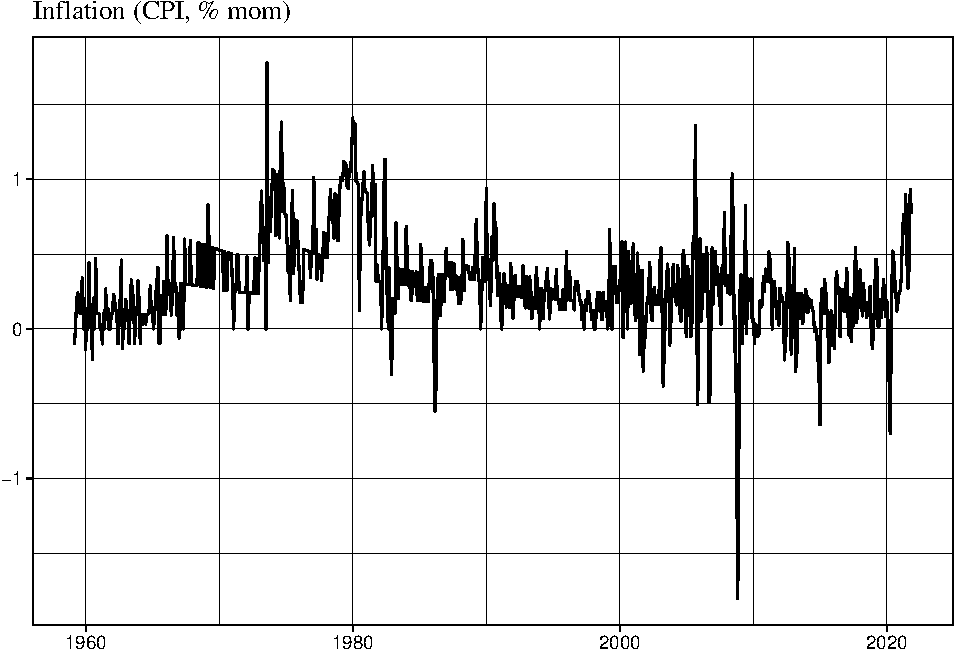
\includegraphics{Trabalho_Econo4_Q2_files/figure-latex/unnamed-chunk-5-1.pdf}

Now, we shall start the estimations.

\hypertarget{ar}{%
\subsubsection{AR}\label{ar}}

In order to get some idea of what the order of our AR(p) process is, we
plot the partial autocorrelation of the inflation series for a
particular window.

\begin{Shaded}
\begin{Highlighting}[]
\CommentTok{\# Partial autocorrelation}
\NormalTok{inflation }\SpecialCharTok{\%\textgreater{}\%}
    \FunctionTok{window}\NormalTok{(}\AttributeTok{start =} \FunctionTok{start}\NormalTok{(inflation), }\AttributeTok{end =} \FunctionTok{start}\NormalTok{(inflation) }\SpecialCharTok{+}
        \FunctionTok{c}\NormalTok{(}\DecValTok{0}\NormalTok{, }\DecValTok{492}\NormalTok{)) }\SpecialCharTok{\%\textgreater{}\%}
    \FunctionTok{Pacf}\NormalTok{(}\AttributeTok{lag.max =} \DecValTok{24}\NormalTok{, }\AttributeTok{plot =}\NormalTok{ T)}
\end{Highlighting}
\end{Shaded}

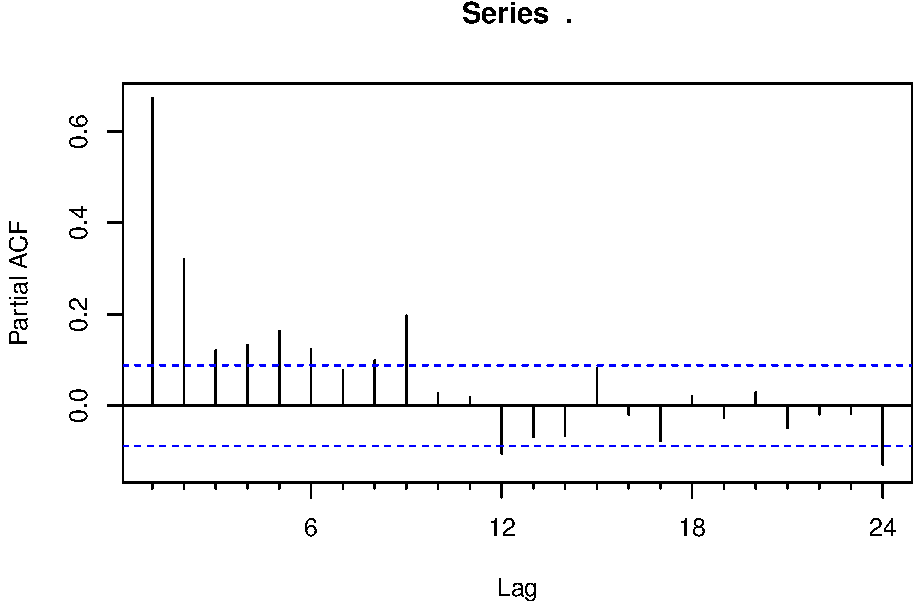
\includegraphics{Trabalho_Econo4_Q2_files/figure-latex/unnamed-chunk-6-1.pdf}

We believe that a maximum lag of 24 is more than reasonable. Then, the
determine the actual order p based on the BIC.

\begin{Shaded}
\begin{Highlighting}[]
\CommentTok{\# Function for calculating the BIC for AR models}
\NormalTok{BIC.ar }\OtherTok{\textless{}{-}} \ControlFlowTok{function}\NormalTok{(model) \{}

\NormalTok{    ssr }\OtherTok{\textless{}{-}} \FunctionTok{sum}\NormalTok{(model}\SpecialCharTok{$}\NormalTok{resid}\SpecialCharTok{\^{}}\DecValTok{2}\NormalTok{, }\AttributeTok{na.rm =}\NormalTok{ T)}
\NormalTok{    t }\OtherTok{\textless{}{-}} \FunctionTok{sum}\NormalTok{(}\SpecialCharTok{!}\FunctionTok{is.na}\NormalTok{(model}\SpecialCharTok{$}\NormalTok{resid))}
\NormalTok{    npar }\OtherTok{\textless{}{-}} \FunctionTok{length}\NormalTok{(model}\SpecialCharTok{$}\NormalTok{ar) }\SpecialCharTok{+} \DecValTok{1}

    \FunctionTok{return}\NormalTok{(}\FunctionTok{c}\NormalTok{(}\AttributeTok{p =}\NormalTok{ model}\SpecialCharTok{$}\NormalTok{order, }\AttributeTok{BIC =} \FunctionTok{log}\NormalTok{(ssr}\SpecialCharTok{/}\NormalTok{t) }\SpecialCharTok{+}\NormalTok{ npar }\SpecialCharTok{*} \FunctionTok{log}\NormalTok{(t)}\SpecialCharTok{/}\NormalTok{t))}
\NormalTok{\}}
\end{Highlighting}
\end{Shaded}

We proceed with a rolling window one-step-ahead forecast, in which we
choose the optimal order of the AR in each window of estimation.

\begin{Shaded}
\begin{Highlighting}[]
\CommentTok{\# Rolling window forecasting}
\NormalTok{rolling\_window }\OtherTok{\textless{}{-}} \DecValTok{492}
\NormalTok{p.max }\OtherTok{\textless{}{-}} \DecValTok{24}

\NormalTok{forecast1 }\OtherTok{=} \FunctionTok{list}\NormalTok{()}
\NormalTok{popt\_AR }\OtherTok{=} \FunctionTok{data.frame}\NormalTok{(}\AttributeTok{popt =} \FunctionTok{numeric}\NormalTok{(}\DecValTok{261}\NormalTok{))}

\ControlFlowTok{for}\NormalTok{ (a }\ControlFlowTok{in} \DecValTok{0}\SpecialCharTok{:}\NormalTok{(}\FunctionTok{length}\NormalTok{(inflation) }\SpecialCharTok{{-}}\NormalTok{ rolling\_window }\SpecialCharTok{{-}} \DecValTok{1}\NormalTok{)) \{}

    \CommentTok{\# get the window for training the model}
\NormalTok{    train }\OtherTok{=} \FunctionTok{window}\NormalTok{(inflation, }\AttributeTok{start =} \FunctionTok{start}\NormalTok{(inflation) }\SpecialCharTok{+} \FunctionTok{c}\NormalTok{(}\DecValTok{0}\NormalTok{,}
\NormalTok{        a), }\AttributeTok{end =} \FunctionTok{start}\NormalTok{(inflation) }\SpecialCharTok{+} \FunctionTok{c}\NormalTok{(}\DecValTok{0}\NormalTok{, a }\SpecialCharTok{+}\NormalTok{ rolling\_window }\SpecialCharTok{{-}}
        \DecValTok{1}\NormalTok{))}

\NormalTok{    bic.table }\OtherTok{=} \FunctionTok{c}\NormalTok{()}

    \ControlFlowTok{for}\NormalTok{ (p }\ControlFlowTok{in} \DecValTok{0}\SpecialCharTok{:}\NormalTok{p.max) \{}
        \CommentTok{\# calculating the BIC for different orders of the}
        \CommentTok{\# AR(p)}
\NormalTok{        AR }\OtherTok{=} \FunctionTok{ar}\NormalTok{(train, }\AttributeTok{order.max =}\NormalTok{ p, }\AttributeTok{method =} \StringTok{"ols"}\NormalTok{, }\AttributeTok{aic =}\NormalTok{ F)}
\NormalTok{        bic.line }\OtherTok{=} \FunctionTok{BIC.ar}\NormalTok{(AR)}
\NormalTok{        bic.table }\OtherTok{=} \FunctionTok{rbind}\NormalTok{(bic.table, bic.line)}
\NormalTok{    \}}
\NormalTok{    bic.table }\OtherTok{=} \FunctionTok{data.frame}\NormalTok{(bic.table)}

\NormalTok{    p.opt }\OtherTok{=}\NormalTok{ bic.table}\SpecialCharTok{$}\NormalTok{p[}\FunctionTok{which.min}\NormalTok{(bic.table}\SpecialCharTok{$}\NormalTok{BIC)]  }\CommentTok{\# pick the optimal p}

\NormalTok{    popt\_AR}\SpecialCharTok{$}\NormalTok{popt[a }\SpecialCharTok{+} \DecValTok{1}\NormalTok{] }\OtherTok{\textless{}{-}}\NormalTok{ p.opt}

\NormalTok{    AR }\OtherTok{=} \FunctionTok{ar}\NormalTok{(train, }\AttributeTok{order.max =}\NormalTok{ p.opt, }\AttributeTok{method =} \StringTok{"ols"}\NormalTok{, }\AttributeTok{aic =}\NormalTok{ F)  }\CommentTok{\# run the AR model with the optimal p}

\NormalTok{    forecast1[[a }\SpecialCharTok{+} \DecValTok{1}\NormalTok{]] }\OtherTok{=} \FunctionTok{predict}\NormalTok{(AR, }\AttributeTok{n.ahead =} \DecValTok{1}\NormalTok{)}\SpecialCharTok{$}\NormalTok{pred  }\CommentTok{\# one{-}step{-}ahead forecast}
\NormalTok{\}}

\NormalTok{forecasts }\OtherTok{=}\NormalTok{ forecast1 }\SpecialCharTok{\%\textgreater{}\%}
    \FunctionTok{unlist}\NormalTok{() }\SpecialCharTok{\%\textgreater{}\%}
    \FunctionTok{ts}\NormalTok{(}\AttributeTok{start =} \FunctionTok{start}\NormalTok{(forecast1[[}\DecValTok{1}\NormalTok{]]), }\AttributeTok{frequency =} \FunctionTok{frequency}\NormalTok{(forecast1[[}\DecValTok{1}\NormalTok{]]))}
\end{Highlighting}
\end{Shaded}

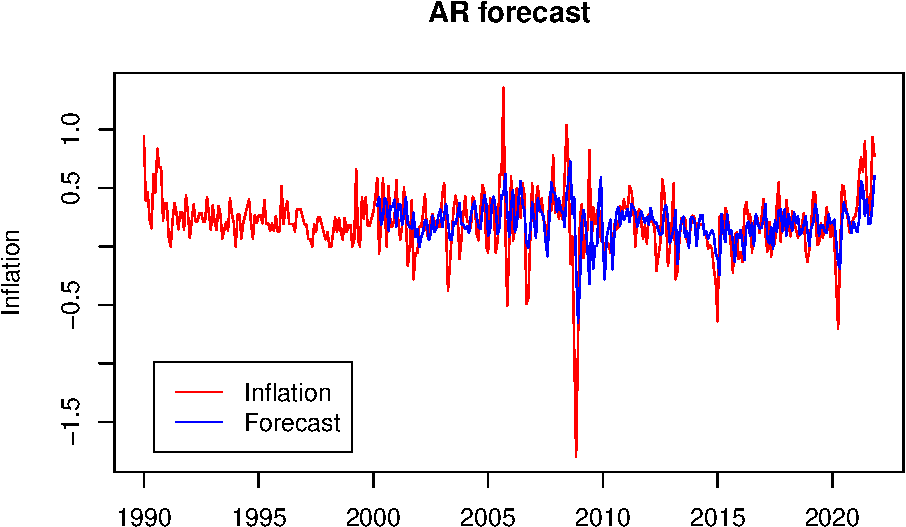
\includegraphics{Trabalho_Econo4_Q2_files/figure-latex/unnamed-chunk-9-1.pdf}

\hypertarget{ar-pc}{%
\subsubsection{AR + PC}\label{ar-pc}}

\begin{enumerate}
\def\labelenumi{\arabic{enumi}.}
\tightlist
\item
  PCA
\end{enumerate}

We do a Principal Component Analysis (PCA). Note that we must center and
scale the data, since the series are in different scales.

\begin{Shaded}
\begin{Highlighting}[]
\CommentTok{\# PCA}
\NormalTok{pca }\OtherTok{=}\NormalTok{ data }\SpecialCharTok{\%\textgreater{}\%}
    \FunctionTok{select}\NormalTok{(}\SpecialCharTok{{-}}\NormalTok{CPIAUCSL, }\SpecialCharTok{{-}}\NormalTok{date) }\SpecialCharTok{\%\textgreater{}\%}
    \FunctionTok{prcomp}\NormalTok{(}\AttributeTok{center =} \ConstantTok{TRUE}\NormalTok{, }\AttributeTok{scale =} \ConstantTok{TRUE}\NormalTok{)}
\end{Highlighting}
\end{Shaded}

\begin{enumerate}
\def\labelenumi{\arabic{enumi}.}
\setcounter{enumi}{1}
\tightlist
\item
  Select PCs
\end{enumerate}

We can, then, choose the number of factors \(k\) and select the first
\(k\) PCs. As seen in Question 1, there are different ways to choose the
number of factors. We look at 3 common criterion (rule of thumb,
informal way and biggest drop), but we opt for the rule of thumb as it
seems to be the most parsimonious in this case.

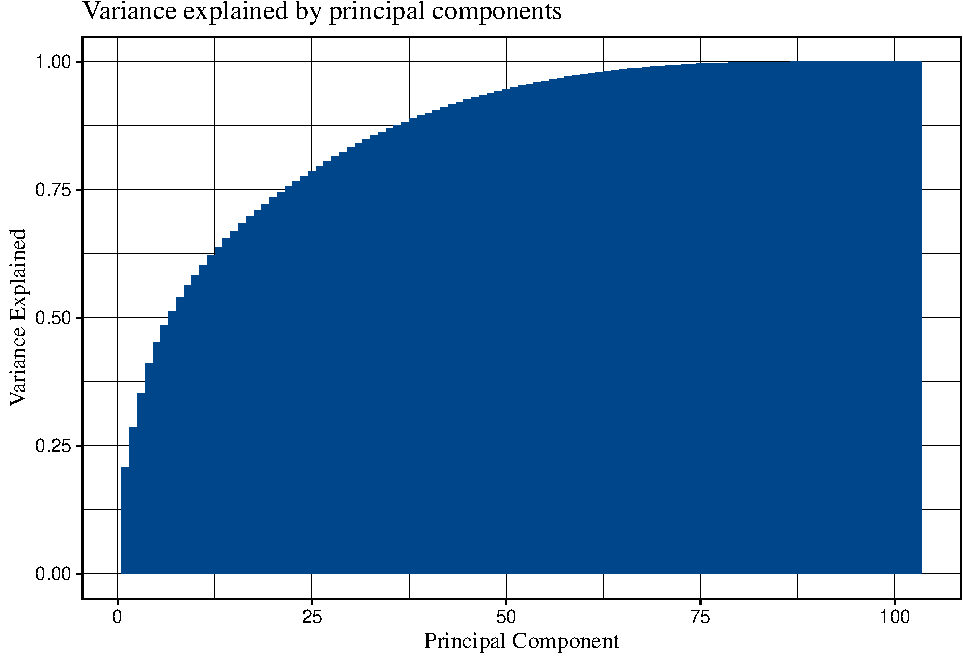
\includegraphics{Trabalho_Econo4_Q2_files/figure-latex/unnamed-chunk-11-1.pdf}

\begin{Shaded}
\begin{Highlighting}[]
\CommentTok{\# Choosing the number of PCs}

\CommentTok{\# Rule of thumb (3\%)}

\NormalTok{pca.var.prop }\SpecialCharTok{\%\textgreater{}\%}
    \FunctionTok{filter}\NormalTok{(var.prop }\SpecialCharTok{\textgreater{}=} \FloatTok{0.03}\NormalTok{) }\SpecialCharTok{\%\textgreater{}\%}
    \FunctionTok{nrow}\NormalTok{() }\SpecialCharTok{\%\textgreater{}\%}
    \FunctionTok{paste}\NormalTok{(}\StringTok{"(rule of thumb)"}\NormalTok{)}
\end{Highlighting}
\end{Shaded}

\begin{verbatim}
## [1] "6 (rule of thumb)"
\end{verbatim}

\begin{Shaded}
\begin{Highlighting}[]
\CommentTok{\# Informal way (90\%)}

\NormalTok{pca.var.prop }\SpecialCharTok{\%\textgreater{}\%}
    \FunctionTok{filter}\NormalTok{(var.prop.cum }\SpecialCharTok{\textless{}=} \FloatTok{0.9}\NormalTok{) }\SpecialCharTok{\%\textgreater{}\%}
    \FunctionTok{nrow}\NormalTok{() }\SpecialCharTok{\%\textgreater{}\%}
    \FunctionTok{paste}\NormalTok{(}\StringTok{"(informal way)"}\NormalTok{)}
\end{Highlighting}
\end{Shaded}

\begin{verbatim}
## [1] "40 (informal way)"
\end{verbatim}

\begin{Shaded}
\begin{Highlighting}[]
\CommentTok{\# Biggest drop}

\NormalTok{(}\FunctionTok{lag}\NormalTok{(pca.var.prop}\SpecialCharTok{$}\NormalTok{var.prop)}\SpecialCharTok{/}\NormalTok{pca.var.prop}\SpecialCharTok{$}\NormalTok{var.prop) }\SpecialCharTok{\%\textgreater{}\%}
    \FunctionTok{which.max}\NormalTok{() }\SpecialCharTok{\%\textgreater{}\%}
    \SpecialCharTok{{-}}\DecValTok{1} \SpecialCharTok{\%\textgreater{}\%}
    \FunctionTok{paste}\NormalTok{(}\StringTok{"(biggest drop)"}\NormalTok{)}
\end{Highlighting}
\end{Shaded}

\begin{verbatim}
## [1] "102 (biggest drop)"
\end{verbatim}

\begin{Shaded}
\begin{Highlighting}[]
\CommentTok{\# Using the rule of thumb}
\NormalTok{n\_pc }\OtherTok{=}\NormalTok{ pca.var.prop }\SpecialCharTok{\%\textgreater{}\%}
    \FunctionTok{filter}\NormalTok{(var.prop }\SpecialCharTok{\textgreater{}=} \FloatTok{0.03}\NormalTok{) }\SpecialCharTok{\%\textgreater{}\%}
    \FunctionTok{nrow}\NormalTok{()}
\end{Highlighting}
\end{Shaded}

\begin{enumerate}
\def\labelenumi{\arabic{enumi}.}
\setcounter{enumi}{2}
\tightlist
\item
  Regression
\end{enumerate}

Given the number of factors, the order of the autoregressive component
is determined by BIC in each rolling window.

\begin{Shaded}
\begin{Highlighting}[]
\CommentTok{\# Get the factor from the PCA}
\NormalTok{Factors }\OtherTok{=}\NormalTok{ pca}\SpecialCharTok{$}\NormalTok{x[, }\DecValTok{1}\SpecialCharTok{:}\NormalTok{n\_pc]}

\CommentTok{\# Create the data matrix with the factors}
\NormalTok{variables }\OtherTok{=} \FunctionTok{cbind}\NormalTok{(inflation, Factors)}

\NormalTok{variables\_withdate }\OtherTok{=}\NormalTok{ variables }\SpecialCharTok{\%\textgreater{}\%}
    \FunctionTok{bind\_cols}\NormalTok{(}\AttributeTok{date =} \FunctionTok{as.Date.yearmon}\NormalTok{(}\FunctionTok{time}\NormalTok{(inflation))) }\SpecialCharTok{\%\textgreater{}\%}
    \FunctionTok{setNames}\NormalTok{(}\FunctionTok{c}\NormalTok{(}\StringTok{"inflation"}\NormalTok{, }\FunctionTok{colnames}\NormalTok{(Factors), }\StringTok{"date"}\NormalTok{))}
\end{Highlighting}
\end{Shaded}

We proceed with the rolling window one-step-ahead forecast.

\begin{Shaded}
\begin{Highlighting}[]
\CommentTok{\# Function for creating the proper data matrix based on the}
\CommentTok{\# regression formula}

\CommentTok{\# Instead of manually creating data matrix, we use the}
\CommentTok{\# dynlm() function and get only the $model component}
\NormalTok{create\_datamatrix }\OtherTok{=} \ControlFlowTok{function}\NormalTok{(train, p.opt) \{}
\NormalTok{    new }\OtherTok{=} \FunctionTok{dynlm}\NormalTok{(inflation }\SpecialCharTok{\textasciitilde{}} \FunctionTok{L}\NormalTok{(inflation, }\DecValTok{1}\SpecialCharTok{:}\NormalTok{p.opt) }\SpecialCharTok{+} \FunctionTok{L}\NormalTok{(train[,}
        \SpecialCharTok{{-}}\DecValTok{1}\NormalTok{], }\DecValTok{1}\NormalTok{), }\AttributeTok{data =} \FunctionTok{ts}\NormalTok{(}\FunctionTok{rbind}\NormalTok{(train, }\DecValTok{0}\NormalTok{), }\AttributeTok{start =} \FunctionTok{start}\NormalTok{(train),}
        \AttributeTok{frequency =} \FunctionTok{frequency}\NormalTok{(train)))}
\NormalTok{    new }\OtherTok{=}\NormalTok{ new}\SpecialCharTok{$}\NormalTok{model }\SpecialCharTok{\%\textgreater{}\%}
        \FunctionTok{tail}\NormalTok{(}\DecValTok{1}\NormalTok{) }\SpecialCharTok{\%\textgreater{}\%}
        \FunctionTok{select}\NormalTok{(}\SpecialCharTok{{-}}\NormalTok{inflation) }\SpecialCharTok{\%\textgreater{}\%}
        \FunctionTok{as.matrix}\NormalTok{()}
    \FunctionTok{return}\NormalTok{(new)}
\NormalTok{\}}
\end{Highlighting}
\end{Shaded}

\begin{Shaded}
\begin{Highlighting}[]
\CommentTok{\# Rolling window forecasting}
\NormalTok{rolling\_window }\OtherTok{\textless{}{-}} \DecValTok{492}
\NormalTok{p.max }\OtherTok{\textless{}{-}} \DecValTok{24}

\NormalTok{forecast1 }\OtherTok{=} \FunctionTok{list}\NormalTok{()}
\NormalTok{coefficients\_pc1 }\OtherTok{\textless{}{-}} \FunctionTok{list}\NormalTok{()}

\CommentTok{\# set up parallel computation}
\FunctionTok{registerDoFuture}\NormalTok{()}
\FunctionTok{plan}\NormalTok{(}\StringTok{"multisession"}\NormalTok{, }\AttributeTok{workers =} \DecValTok{3}\NormalTok{)  }\CommentTok{\# use 3 cores }

\CommentTok{\# Loop}
\NormalTok{forecast1 }\OtherTok{=} \FunctionTok{foreach}\NormalTok{(}\AttributeTok{a =} \DecValTok{0}\SpecialCharTok{:}\NormalTok{(}\FunctionTok{length}\NormalTok{(inflation) }\SpecialCharTok{{-}}\NormalTok{ rolling\_window }\SpecialCharTok{{-}}
    \DecValTok{1}\NormalTok{)) }\SpecialCharTok{\%dorng\%}\NormalTok{ \{}

\NormalTok{    train }\OtherTok{=} \FunctionTok{window}\NormalTok{(variables, }\AttributeTok{start =} \FunctionTok{start}\NormalTok{(inflation) }\SpecialCharTok{+} \FunctionTok{c}\NormalTok{(}\DecValTok{0}\NormalTok{,}
\NormalTok{        a), }\AttributeTok{end =} \FunctionTok{start}\NormalTok{(inflation) }\SpecialCharTok{+} \FunctionTok{c}\NormalTok{(}\DecValTok{0}\NormalTok{, a }\SpecialCharTok{+}\NormalTok{ rolling\_window }\SpecialCharTok{{-}}
        \DecValTok{1}\NormalTok{))}

\NormalTok{    bic.table }\OtherTok{=} \FunctionTok{rep}\NormalTok{(}\ConstantTok{NA}\NormalTok{, p.max)}

    \ControlFlowTok{for}\NormalTok{ (p }\ControlFlowTok{in} \DecValTok{1}\SpecialCharTok{:}\NormalTok{p.max) \{}
        \CommentTok{\# calculating the BIC for different orders of the}
        \CommentTok{\# AR(p)}
\NormalTok{        AR\_PC }\OtherTok{=} \FunctionTok{dynlm}\NormalTok{(inflation }\SpecialCharTok{\textasciitilde{}} \FunctionTok{L}\NormalTok{(inflation, }\DecValTok{1}\SpecialCharTok{:}\NormalTok{p) }\SpecialCharTok{+} \FunctionTok{L}\NormalTok{(train[,}
            \SpecialCharTok{{-}}\DecValTok{1}\NormalTok{], }\DecValTok{1}\NormalTok{), }\AttributeTok{data =}\NormalTok{ train)}
\NormalTok{        bic.table[p] }\OtherTok{=} \FunctionTok{BIC}\NormalTok{(AR\_PC)}
\NormalTok{    \}}

\NormalTok{    p.opt }\OtherTok{=} \FunctionTok{which.min}\NormalTok{(bic.table)  }\CommentTok{\# pick the optimal p}

\NormalTok{    AR\_PC }\OtherTok{=} \FunctionTok{dynlm}\NormalTok{(inflation }\SpecialCharTok{\textasciitilde{}} \FunctionTok{L}\NormalTok{(inflation, }\DecValTok{1}\SpecialCharTok{:}\NormalTok{p.opt) }\SpecialCharTok{+} \FunctionTok{L}\NormalTok{(train[,}
        \SpecialCharTok{{-}}\DecValTok{1}\NormalTok{], }\DecValTok{1}\NormalTok{), }\AttributeTok{data =}\NormalTok{ train)  }\CommentTok{\# run the AR{-}PC model with the optimal p}

\NormalTok{    new }\OtherTok{=} \FunctionTok{create\_datamatrix}\NormalTok{(train, p.opt)}

\NormalTok{    result }\OtherTok{=}\NormalTok{ AR\_PC}\SpecialCharTok{$}\NormalTok{coefficients }\SpecialCharTok{\%*\%} \FunctionTok{c}\NormalTok{(}\DecValTok{1}\NormalTok{, new)  }\CommentTok{\# one{-}step{-}ahead forecast}
\NormalTok{    result}
\NormalTok{\}}

\NormalTok{forecast1 }\OtherTok{=}\NormalTok{ forecast1 }\SpecialCharTok{\%\textgreater{}\%}
    \FunctionTok{unlist}\NormalTok{() }\SpecialCharTok{\%\textgreater{}\%}
    \FunctionTok{ts}\NormalTok{(}\AttributeTok{start =} \FunctionTok{start}\NormalTok{(inflation) }\SpecialCharTok{+} \FunctionTok{c}\NormalTok{(}\DecValTok{0}\NormalTok{, rolling\_window), }\AttributeTok{frequency =} \FunctionTok{frequency}\NormalTok{(inflation))}


\CommentTok{\# Loop to get coefficients}
\NormalTok{coefficients\_pc1 }\OtherTok{=} \FunctionTok{foreach}\NormalTok{(}\AttributeTok{a =} \DecValTok{0}\SpecialCharTok{:}\NormalTok{(}\FunctionTok{length}\NormalTok{(inflation) }\SpecialCharTok{{-}}\NormalTok{ rolling\_window }\SpecialCharTok{{-}}
    \DecValTok{1}\NormalTok{)) }\SpecialCharTok{\%dorng\%}\NormalTok{ \{}

\NormalTok{    train }\OtherTok{=} \FunctionTok{window}\NormalTok{(variables, }\AttributeTok{start =} \FunctionTok{start}\NormalTok{(inflation) }\SpecialCharTok{+} \FunctionTok{c}\NormalTok{(}\DecValTok{0}\NormalTok{,}
\NormalTok{        a), }\AttributeTok{end =} \FunctionTok{start}\NormalTok{(inflation) }\SpecialCharTok{+} \FunctionTok{c}\NormalTok{(}\DecValTok{0}\NormalTok{, a }\SpecialCharTok{+}\NormalTok{ rolling\_window }\SpecialCharTok{{-}}
        \DecValTok{1}\NormalTok{))}

\NormalTok{    bic.table }\OtherTok{=} \FunctionTok{rep}\NormalTok{(}\ConstantTok{NA}\NormalTok{, p.max)}

    \ControlFlowTok{for}\NormalTok{ (p }\ControlFlowTok{in} \DecValTok{1}\SpecialCharTok{:}\NormalTok{p.max) \{}
        \CommentTok{\# calculating the BIC for different orders of the}
        \CommentTok{\# AR(p)}
\NormalTok{        AR\_PC }\OtherTok{=} \FunctionTok{dynlm}\NormalTok{(inflation }\SpecialCharTok{\textasciitilde{}} \FunctionTok{L}\NormalTok{(inflation, }\DecValTok{1}\SpecialCharTok{:}\NormalTok{p) }\SpecialCharTok{+} \FunctionTok{L}\NormalTok{(train[,}
            \SpecialCharTok{{-}}\DecValTok{1}\NormalTok{], }\DecValTok{1}\NormalTok{), }\AttributeTok{data =}\NormalTok{ train)}
\NormalTok{        bic.table[p] }\OtherTok{=} \FunctionTok{BIC}\NormalTok{(AR\_PC)}
\NormalTok{    \}}

\NormalTok{    p.opt }\OtherTok{=} \FunctionTok{which.min}\NormalTok{(bic.table)  }\CommentTok{\# pick the optimal p}

\NormalTok{    AR\_PC }\OtherTok{=} \FunctionTok{dynlm}\NormalTok{(inflation }\SpecialCharTok{\textasciitilde{}} \FunctionTok{L}\NormalTok{(inflation, }\DecValTok{1}\SpecialCharTok{:}\NormalTok{p.opt) }\SpecialCharTok{+} \FunctionTok{L}\NormalTok{(train[,}
        \SpecialCharTok{{-}}\DecValTok{1}\NormalTok{], }\DecValTok{1}\NormalTok{), }\AttributeTok{data =}\NormalTok{ train)  }\CommentTok{\# run the AR{-}PC model with the optimal p}

\NormalTok{    result }\OtherTok{=}\NormalTok{ AR\_PC[[}\DecValTok{1}\NormalTok{]]  }\CommentTok{\# one{-}step{-}ahead forecast}
\NormalTok{    result}
\NormalTok{\}}
\end{Highlighting}
\end{Shaded}

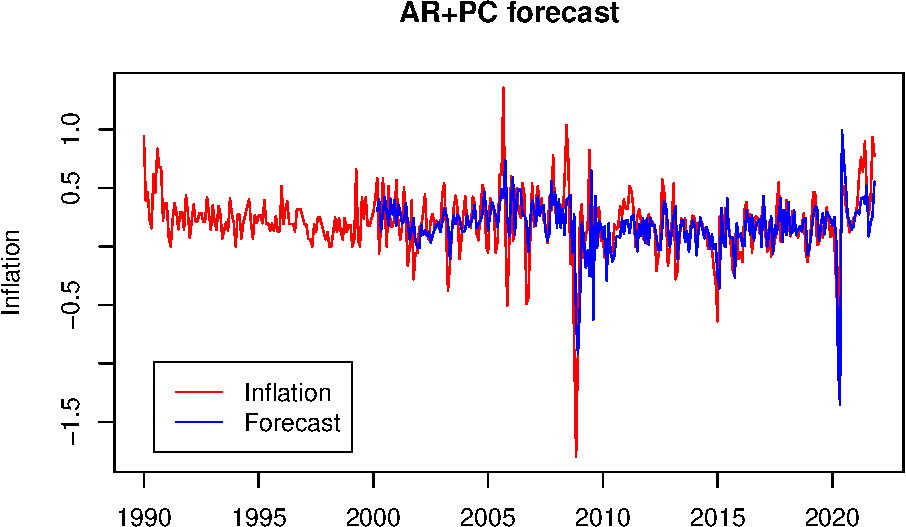
\includegraphics{Trabalho_Econo4_Q2_files/figure-latex/unnamed-chunk-16-1.pdf}

\begin{Shaded}
\begin{Highlighting}[]
\CommentTok{\# Save forecasts}
\NormalTok{forecasts }\OtherTok{=} \FunctionTok{cbind}\NormalTok{(}\AttributeTok{AR =}\NormalTok{ forecasts, }\AttributeTok{AR\_PC =}\NormalTok{ forecast1) }\SpecialCharTok{\%\textgreater{}\%}
    \FunctionTok{as.ts}\NormalTok{()}
\end{Highlighting}
\end{Shaded}

\hypertarget{ridge-regression}{%
\subsubsection{Ridge Regression}\label{ridge-regression}}

We will choose penalty term according to the BIC. However, we must
decide on the number of lags in the model and this criterion is
obviously silent about this issue. Our strategy will be to run the
models with 1, 2, 3 and 4 lags and choose the model with the smallest
MSE.

\begin{Shaded}
\begin{Highlighting}[]
\CommentTok{\# Embedding function that creates n\_lags of all variables}
\CommentTok{\# of a given data frame}
\NormalTok{my\_embed }\OtherTok{=} \ControlFlowTok{function}\NormalTok{(df, }\AttributeTok{n\_lags =} \DecValTok{4}\NormalTok{) \{}
\NormalTok{    Lags }\OtherTok{=} \FunctionTok{list}\NormalTok{()}
\NormalTok{    Lags[[}\DecValTok{1}\NormalTok{]] }\OtherTok{=}\NormalTok{ df }\SpecialCharTok{\%\textgreater{}\%}
        \FunctionTok{select}\NormalTok{(}\SpecialCharTok{{-}}\FunctionTok{contains}\NormalTok{(}\StringTok{"date"}\NormalTok{))}
    \ControlFlowTok{if}\NormalTok{ (n\_lags }\SpecialCharTok{\textgreater{}=} \DecValTok{1}\NormalTok{) \{}
        \ControlFlowTok{for}\NormalTok{ (i }\ControlFlowTok{in} \DecValTok{1}\SpecialCharTok{:}\NormalTok{n\_lags) \{}
\NormalTok{            Lags[[i }\SpecialCharTok{+} \DecValTok{1}\NormalTok{]] }\OtherTok{=}\NormalTok{ df }\SpecialCharTok{\%\textgreater{}\%}
                \FunctionTok{select}\NormalTok{(}\SpecialCharTok{{-}}\FunctionTok{contains}\NormalTok{(}\StringTok{"date"}\NormalTok{)) }\SpecialCharTok{\%\textgreater{}\%}
                \FunctionTok{mutate\_all}\NormalTok{(}\ControlFlowTok{function}\NormalTok{(x) }\FunctionTok{lag}\NormalTok{(x, }\AttributeTok{n =}\NormalTok{ i))}
\NormalTok{        \}}
\NormalTok{    \}}
\NormalTok{    lagged\_data }\OtherTok{=} \FunctionTok{reduce}\NormalTok{(Lags, }\ControlFlowTok{function}\NormalTok{(x, y) \{}
        \FunctionTok{bind\_cols}\NormalTok{(x, y, }\AttributeTok{.name\_repair =} \SpecialCharTok{\textasciitilde{}}\FunctionTok{make.unique}\NormalTok{(.x))}
\NormalTok{    \})}

    \FunctionTok{return}\NormalTok{(lagged\_data)}
\NormalTok{\}}
\end{Highlighting}
\end{Shaded}

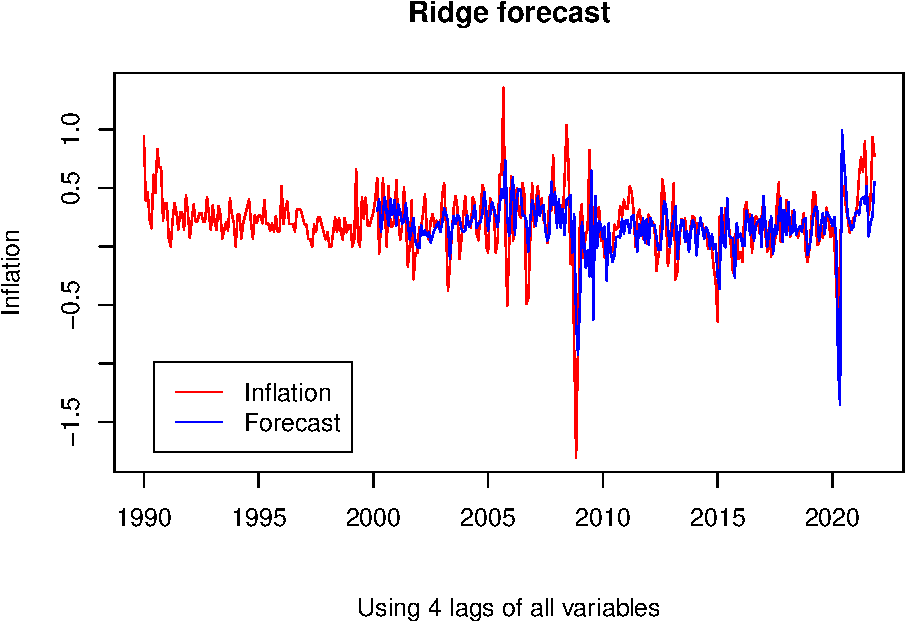
\includegraphics{Trabalho_Econo4_Q2_files/figure-latex/unnamed-chunk-19-1.pdf}

\begin{Shaded}
\begin{Highlighting}[]
\CommentTok{\# Save forecasts}
\NormalTok{forecasts }\OtherTok{=} \FunctionTok{cbind.zoo}\NormalTok{(forecasts, }\AttributeTok{Ridge\_4lags =}\NormalTok{ forecast1) }\SpecialCharTok{\%\textgreater{}\%}
    \FunctionTok{as.ts}\NormalTok{()}
\end{Highlighting}
\end{Shaded}

The forecast of the Ridge regression with 4 lags has a notably bad fit
to the actual inflation series. We noticed that, since the ridge is not
able to give a sparse solution, when there are too many variables, the
estimated model becomes basically an intercept and almost all the other
coefficients are very close to zero (but not zero). Hence, we tested
other (more parsimonious) specifications. When we include the all the
macroeconomics variables - without any lags - and lags of the CPI, we
get a more reasonable result. The results are very robust to the number
of CPI lags, so we keep 4 lags, as initially intended.

\begin{Shaded}
\begin{Highlighting}[]
\FunctionTok{tic}\NormalTok{()}
\CommentTok{\# Rolling window forecasting}
\NormalTok{rolling\_window }\OtherTok{\textless{}{-}} \DecValTok{492}

\CommentTok{\# glmnet parameter}
\NormalTok{my\_alpha }\OtherTok{=} \DecValTok{0}  \CommentTok{\# Ridge}

\NormalTok{forecast1 }\OtherTok{=} \FunctionTok{list}\NormalTok{()}

\CommentTok{\# set up parallel computation}
\FunctionTok{registerDoFuture}\NormalTok{()}
\FunctionTok{plan}\NormalTok{(}\StringTok{"multisession"}\NormalTok{, }\AttributeTok{workers =} \DecValTok{3}\NormalTok{)  }\CommentTok{\# use 3 cores }

\NormalTok{last\_fcst }\OtherTok{=}\NormalTok{ (}\FunctionTok{length}\NormalTok{(inflation) }\SpecialCharTok{{-}}\NormalTok{ rolling\_window)}

\NormalTok{output }\OtherTok{=} \FunctionTok{foreach}\NormalTok{(}\AttributeTok{a =} \DecValTok{1}\SpecialCharTok{:}\NormalTok{last\_fcst) }\SpecialCharTok{\%dorng\%}\NormalTok{ \{}
    \CommentTok{\# get the window for training the model}
\NormalTok{    train }\OtherTok{=}\NormalTok{ data[a}\SpecialCharTok{:}\NormalTok{(a }\SpecialCharTok{+}\NormalTok{ rolling\_window }\SpecialCharTok{{-}} \DecValTok{1}\NormalTok{), ] }\SpecialCharTok{\%\textgreater{}\%}
        \FunctionTok{select}\NormalTok{(}\SpecialCharTok{{-}}\NormalTok{CPIAUCSL)}
\NormalTok{    train\_cpi }\OtherTok{=}\NormalTok{ data[a}\SpecialCharTok{:}\NormalTok{(a }\SpecialCharTok{+}\NormalTok{ rolling\_window }\SpecialCharTok{{-}} \DecValTok{1}\NormalTok{), ] }\SpecialCharTok{\%\textgreater{}\%}
        \FunctionTok{select}\NormalTok{(CPIAUCSL)}
    \CommentTok{\# embed}
\NormalTok{    reg\_data }\OtherTok{=} \FunctionTok{my\_embed}\NormalTok{(train, }\AttributeTok{n\_lags =} \DecValTok{0}\NormalTok{)}
\NormalTok{    cpi\_lags }\OtherTok{=} \FunctionTok{my\_embed}\NormalTok{(train\_cpi, }\AttributeTok{n\_lags =} \DecValTok{4}\NormalTok{)}
    \CommentTok{\# bind the embeded columns with the one{-}step{-}ahead}
    \CommentTok{\# inflation}
\NormalTok{    reg\_data }\OtherTok{=} \FunctionTok{bind\_cols}\NormalTok{(}\AttributeTok{inflation.ahead =} \FunctionTok{lead}\NormalTok{(inflation[a}\SpecialCharTok{:}\NormalTok{(a }\SpecialCharTok{+}
\NormalTok{        rolling\_window }\SpecialCharTok{{-}} \DecValTok{1}\NormalTok{)]), cpi\_lags, reg\_data)}

    \CommentTok{\# Ridge estimation}
\NormalTok{    ic\_ridge }\OtherTok{\textless{}{-}} \FunctionTok{ic.glmnet}\NormalTok{(}\AttributeTok{x =}\NormalTok{ reg\_data }\SpecialCharTok{\%\textgreater{}\%}
        \FunctionTok{na.omit}\NormalTok{() }\SpecialCharTok{\%\textgreater{}\%}
        \FunctionTok{select}\NormalTok{(}\SpecialCharTok{{-}}\NormalTok{inflation.ahead), }\AttributeTok{y =}\NormalTok{ reg\_data }\SpecialCharTok{\%\textgreater{}\%}
        \FunctionTok{na.omit}\NormalTok{() }\SpecialCharTok{\%\textgreater{}\%}
        \FunctionTok{select}\NormalTok{(inflation.ahead) }\SpecialCharTok{\%\textgreater{}\%}
        \FunctionTok{data.matrix}\NormalTok{(), }\AttributeTok{crit =} \StringTok{"bic"}\NormalTok{, }\AttributeTok{alpha =}\NormalTok{ my\_alpha)}
\NormalTok{    ridge }\OtherTok{\textless{}{-}} \FunctionTok{glmnet}\NormalTok{(}\AttributeTok{x =}\NormalTok{ reg\_data }\SpecialCharTok{\%\textgreater{}\%}
        \FunctionTok{na.omit}\NormalTok{() }\SpecialCharTok{\%\textgreater{}\%}
        \FunctionTok{select}\NormalTok{(}\SpecialCharTok{{-}}\NormalTok{inflation.ahead), }\AttributeTok{y =}\NormalTok{ reg\_data }\SpecialCharTok{\%\textgreater{}\%}
        \FunctionTok{na.omit}\NormalTok{() }\SpecialCharTok{\%\textgreater{}\%}
        \FunctionTok{select}\NormalTok{(inflation.ahead) }\SpecialCharTok{\%\textgreater{}\%}
        \FunctionTok{data.matrix}\NormalTok{(), }\AttributeTok{alpha =}\NormalTok{ my\_alpha, }\AttributeTok{lambda =}\NormalTok{ ic\_ridge}\SpecialCharTok{$}\NormalTok{lambda)}

    \CommentTok{\# Prediction}
\NormalTok{    new }\OtherTok{=}\NormalTok{ reg\_data }\SpecialCharTok{\%\textgreater{}\%}
        \FunctionTok{select}\NormalTok{(}\SpecialCharTok{{-}}\NormalTok{inflation.ahead) }\SpecialCharTok{\%\textgreater{}\%}
        \FunctionTok{tail}\NormalTok{(}\DecValTok{1}\NormalTok{)}
\NormalTok{    result1 }\OtherTok{=} \FunctionTok{predict}\NormalTok{(ridge, }\AttributeTok{newx =} \FunctionTok{data.matrix}\NormalTok{(new), }\AttributeTok{s =}\NormalTok{ ic\_ridge}\SpecialCharTok{$}\NormalTok{lambda)}

    \CommentTok{\# Coeficients}
\NormalTok{    result2 }\OtherTok{=} \FunctionTok{coef}\NormalTok{(ridge, }\AttributeTok{s =}\NormalTok{ ic\_ridge}\SpecialCharTok{$}\NormalTok{lambda)}

\NormalTok{    result }\OtherTok{=} \FunctionTok{list}\NormalTok{(}\AttributeTok{forecast1 =}\NormalTok{ result1, }\AttributeTok{coef =}\NormalTok{ result2)}
\NormalTok{    result}
\NormalTok{\}}

\NormalTok{output }\OtherTok{=}\NormalTok{ output }\SpecialCharTok{\%\textgreater{}\%}
    \FunctionTok{transpose}\NormalTok{()}

\NormalTok{forecast1 }\OtherTok{=}\NormalTok{ output}\SpecialCharTok{$}\NormalTok{forecast1 }\SpecialCharTok{\%\textgreater{}\%}
    \FunctionTok{unlist}\NormalTok{() }\SpecialCharTok{\%\textgreater{}\%}
    \FunctionTok{ts}\NormalTok{(}\AttributeTok{start =} \FunctionTok{start}\NormalTok{(inflation) }\SpecialCharTok{+} \FunctionTok{c}\NormalTok{(}\DecValTok{0}\NormalTok{, rolling\_window), }\AttributeTok{frequency =} \FunctionTok{frequency}\NormalTok{(inflation))}

\NormalTok{ridge\_coeficients }\OtherTok{=}\NormalTok{ output}\SpecialCharTok{$}\NormalTok{coef }\SpecialCharTok{\%\textgreater{}\%}
    \FunctionTok{reduce}\NormalTok{(cbind) }\SpecialCharTok{\%\textgreater{}\%}
    \FunctionTok{as.matrix}\NormalTok{()}

\FunctionTok{toc}\NormalTok{()}
\end{Highlighting}
\end{Shaded}

\begin{verbatim}
## 115.872 sec elapsed
\end{verbatim}

\begin{Shaded}
\begin{Highlighting}[]
\NormalTok{beepr}\SpecialCharTok{::}\FunctionTok{beep}\NormalTok{()}
\end{Highlighting}
\end{Shaded}

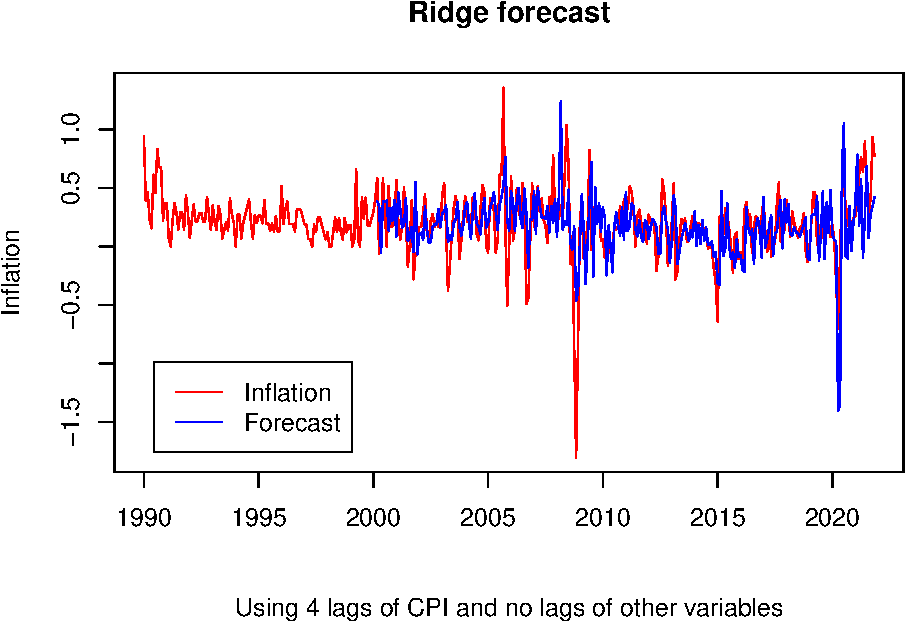
\includegraphics{Trabalho_Econo4_Q2_files/figure-latex/unnamed-chunk-21-1.pdf}

\begin{Shaded}
\begin{Highlighting}[]
\CommentTok{\# Save forecasts}
\NormalTok{forecasts }\OtherTok{=} \FunctionTok{cbind.zoo}\NormalTok{(forecasts, }\AttributeTok{Ridge =}\NormalTok{ forecast1) }\SpecialCharTok{\%\textgreater{}\%}
    \FunctionTok{as.ts}\NormalTok{()}
\end{Highlighting}
\end{Shaded}

\hypertarget{lasso-regression}{%
\subsubsection{LASSO Regression}\label{lasso-regression}}

\begin{Shaded}
\begin{Highlighting}[]
\FunctionTok{tic}\NormalTok{()}
\CommentTok{\# Rolling window forecasting}
\NormalTok{rolling\_window }\OtherTok{\textless{}{-}} \DecValTok{492}

\CommentTok{\# glmnet parameter}
\NormalTok{my\_alpha }\OtherTok{=} \DecValTok{1}  \CommentTok{\# LASSO}

\NormalTok{forecast1 }\OtherTok{=} \FunctionTok{list}\NormalTok{()}
\NormalTok{coefficients\_lasso }\OtherTok{=} \FunctionTok{list}\NormalTok{()}


\ControlFlowTok{for}\NormalTok{ (a }\ControlFlowTok{in} \DecValTok{1}\SpecialCharTok{:}\NormalTok{(}\FunctionTok{length}\NormalTok{(inflation) }\SpecialCharTok{{-}}\NormalTok{ rolling\_window)) \{}
    \CommentTok{\# get the window for training the model}
\NormalTok{    train }\OtherTok{=}\NormalTok{ data[a}\SpecialCharTok{:}\NormalTok{(a }\SpecialCharTok{+}\NormalTok{ rolling\_window }\SpecialCharTok{{-}} \DecValTok{1}\NormalTok{), ]}
    \CommentTok{\# embed}
\NormalTok{    reg\_data }\OtherTok{=} \FunctionTok{my\_embed}\NormalTok{(train)}
    \CommentTok{\# bind the embeded columns with the one{-}step{-}ahead}
    \CommentTok{\# inflation}
\NormalTok{    reg\_data }\OtherTok{=} \FunctionTok{bind\_cols}\NormalTok{(}\AttributeTok{inflation.ahead =} \FunctionTok{lead}\NormalTok{(inflation[a}\SpecialCharTok{:}\NormalTok{(a }\SpecialCharTok{+}
\NormalTok{        rolling\_window }\SpecialCharTok{{-}} \DecValTok{1}\NormalTok{)]), reg\_data)}

    \CommentTok{\# Ridge estimation}
\NormalTok{    ic\_lasso }\OtherTok{\textless{}{-}} \FunctionTok{ic.glmnet}\NormalTok{(}\AttributeTok{x =}\NormalTok{ reg\_data }\SpecialCharTok{\%\textgreater{}\%}
        \FunctionTok{na.omit}\NormalTok{() }\SpecialCharTok{\%\textgreater{}\%}
        \FunctionTok{select}\NormalTok{(}\SpecialCharTok{{-}}\NormalTok{inflation.ahead), }\AttributeTok{y =}\NormalTok{ reg\_data }\SpecialCharTok{\%\textgreater{}\%}
        \FunctionTok{na.omit}\NormalTok{() }\SpecialCharTok{\%\textgreater{}\%}
        \FunctionTok{select}\NormalTok{(inflation.ahead) }\SpecialCharTok{\%\textgreater{}\%}
        \FunctionTok{data.matrix}\NormalTok{(), }\AttributeTok{crit =} \StringTok{"bic"}\NormalTok{, }\AttributeTok{alpha =}\NormalTok{ my\_alpha)}
\NormalTok{    lasso }\OtherTok{\textless{}{-}} \FunctionTok{glmnet}\NormalTok{(}\AttributeTok{x =}\NormalTok{ reg\_data }\SpecialCharTok{\%\textgreater{}\%}
        \FunctionTok{na.omit}\NormalTok{() }\SpecialCharTok{\%\textgreater{}\%}
        \FunctionTok{select}\NormalTok{(}\SpecialCharTok{{-}}\NormalTok{inflation.ahead), }\AttributeTok{y =}\NormalTok{ reg\_data }\SpecialCharTok{\%\textgreater{}\%}
        \FunctionTok{na.omit}\NormalTok{() }\SpecialCharTok{\%\textgreater{}\%}
        \FunctionTok{select}\NormalTok{(inflation.ahead) }\SpecialCharTok{\%\textgreater{}\%}
        \FunctionTok{data.matrix}\NormalTok{(), }\AttributeTok{alpha =}\NormalTok{ my\_alpha, }\AttributeTok{lambda =}\NormalTok{ ic\_lasso}\SpecialCharTok{$}\NormalTok{lambda)}

    \CommentTok{\# Prediction}
\NormalTok{    new }\OtherTok{=}\NormalTok{ reg\_data }\SpecialCharTok{\%\textgreater{}\%}
        \FunctionTok{select}\NormalTok{(}\SpecialCharTok{{-}}\NormalTok{inflation.ahead) }\SpecialCharTok{\%\textgreater{}\%}
        \FunctionTok{tail}\NormalTok{(}\DecValTok{1}\NormalTok{)}
\NormalTok{    forecast1[a] }\OtherTok{=} \FunctionTok{predict}\NormalTok{(lasso, }\AttributeTok{newx =} \FunctionTok{data.matrix}\NormalTok{(new), }\AttributeTok{s =}\NormalTok{ ic\_lasso}\SpecialCharTok{$}\NormalTok{lambda)}

    \CommentTok{\# Coefficients}
\NormalTok{    coefficients\_lasso[a] }\OtherTok{=} \FunctionTok{coef}\NormalTok{(lasso)}

\NormalTok{\}}

\NormalTok{forecast1 }\OtherTok{=}\NormalTok{ forecast1 }\SpecialCharTok{\%\textgreater{}\%}
    \FunctionTok{unlist}\NormalTok{() }\SpecialCharTok{\%\textgreater{}\%}
    \FunctionTok{ts}\NormalTok{(}\AttributeTok{start =} \FunctionTok{start}\NormalTok{(inflation) }\SpecialCharTok{+} \FunctionTok{c}\NormalTok{(}\DecValTok{0}\NormalTok{, rolling\_window), }\AttributeTok{frequency =} \FunctionTok{frequency}\NormalTok{(inflation))}

\FunctionTok{toc}\NormalTok{()}
\end{Highlighting}
\end{Shaded}

\begin{verbatim}
## 37.407 sec elapsed
\end{verbatim}

\begin{Shaded}
\begin{Highlighting}[]
\NormalTok{beepr}\SpecialCharTok{::}\FunctionTok{beep}\NormalTok{()}
\end{Highlighting}
\end{Shaded}

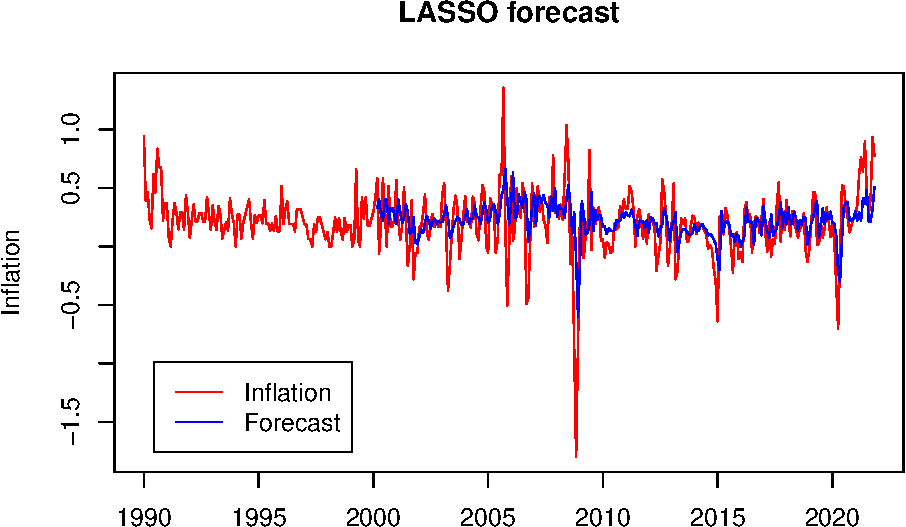
\includegraphics{Trabalho_Econo4_Q2_files/figure-latex/unnamed-chunk-23-1.pdf}

\begin{Shaded}
\begin{Highlighting}[]
\CommentTok{\# Save forecasts}
\NormalTok{forecasts }\OtherTok{=} \FunctionTok{cbind.zoo}\NormalTok{(forecasts, }\AttributeTok{LASSO =}\NormalTok{ forecast1) }\SpecialCharTok{\%\textgreater{}\%}
    \FunctionTok{as.ts}\NormalTok{()}
\end{Highlighting}
\end{Shaded}

\hypertarget{item-a}{%
\subsection{Item A}\label{item-a}}

\begin{Shaded}
\begin{Highlighting}[]
\CommentTok{\# Forecasting error}
\NormalTok{error }\OtherTok{=}\NormalTok{ inflation }\SpecialCharTok{{-}}\NormalTok{ forecasts}
\NormalTok{cum\_error }\OtherTok{=} \FunctionTok{sapply}\NormalTok{(error, }\ControlFlowTok{function}\NormalTok{(x) \{}
\NormalTok{    x}\SpecialCharTok{\^{}}\DecValTok{2} \SpecialCharTok{\%\textgreater{}\%}
        \FunctionTok{cumsum}\NormalTok{()}
\NormalTok{\}) }\SpecialCharTok{\%\textgreater{}\%}
    \FunctionTok{bind\_cols}\NormalTok{(}\AttributeTok{date =} \FunctionTok{as.Date.yearmon}\NormalTok{(}\FunctionTok{time}\NormalTok{(error))) }\SpecialCharTok{\%\textgreater{}\%}
    \FunctionTok{setNames}\NormalTok{(}\FunctionTok{c}\NormalTok{(}\StringTok{"AR"}\NormalTok{, }\StringTok{"AR+PC"}\NormalTok{, }\StringTok{"Ridge (4 lags)"}\NormalTok{, }\StringTok{"Ridge"}\NormalTok{, }\StringTok{"LASSO"}\NormalTok{,}
        \StringTok{"date"}\NormalTok{))}


\CommentTok{\# cum\_error = sapply(error, function(x)\{x\^{}2 \%\textgreater{}\% cumsum()\})}
\CommentTok{\# \%\textgreater{}\% bind\_cols(date = as.Date.yearmon(time(error))) \%\textgreater{}\%}
\CommentTok{\# setNames( c(\textquotesingle{}AR\textquotesingle{}, \textquotesingle{}AR+PC\textquotesingle{}, \textquotesingle{}Ridge\textquotesingle{}, \textquotesingle{}LASSO\textquotesingle{}, \textquotesingle{}date\textquotesingle{} ) )}
\end{Highlighting}
\end{Shaded}

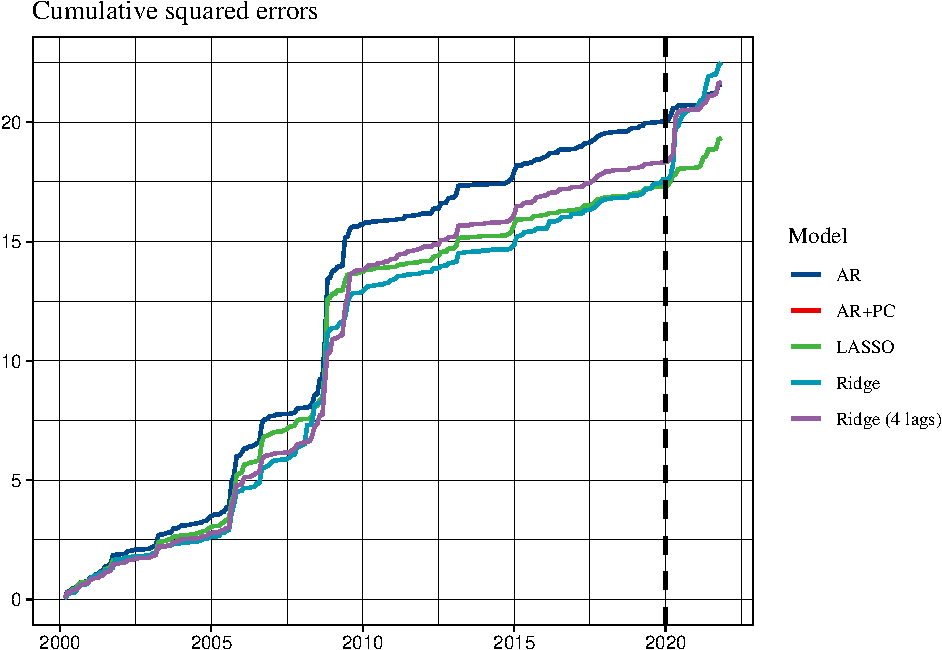
\includegraphics{Trabalho_Econo4_Q2_files/figure-latex/unnamed-chunk-26-1.pdf}

\hypertarget{item-b}{%
\subsection{Item B}\label{item-b}}

We will follow the FRED-MD classification of variables into 8 groups:
(i) output and income; (ii) labor market; (iii) housing; (iv)
consumption,orders and inventories; (v) money and credit; (vi) interest
and exchange rates; (vii) prices; and (viii) stock market. We are adding
a ninth group called (ix) lags, with the lagged inflation series.

\begin{Shaded}
\begin{Highlighting}[]
\CommentTok{\# Get FRED groups groups = read\_xlsx(\textquotesingle{}C:\textbackslash{}\textbackslash{}Users\textbackslash{}\textbackslash{}Caio}
\CommentTok{\# Garzeri\textbackslash{}\textbackslash{}OneDrive {-} puc{-}rio.br\textbackslash{}\textbackslash{}Econometria}
\CommentTok{\# IV\textbackslash{}\textbackslash{}AssignmentEconometricsIV\textbackslash{}\textbackslash{}data\textbackslash{}\textbackslash{}FRED{-}MD\_updated\_appendix.xlsx\textquotesingle{})}
\NormalTok{groups }\OtherTok{=} \FunctionTok{read\_xlsx}\NormalTok{(}\StringTok{"data/FRED{-}MD\_updated\_appendix.xlsx"}\NormalTok{)}
\NormalTok{groups }\OtherTok{\textless{}{-}}\NormalTok{ groups }\SpecialCharTok{\%\textgreater{}\%}
    \FunctionTok{select}\NormalTok{(fred, group)}


\CommentTok{\# Change some names manually because they have minor}
\CommentTok{\# differences with the variable names in existing dataframe}
\NormalTok{groups}\SpecialCharTok{$}\NormalTok{fred[groups}\SpecialCharTok{$}\NormalTok{fred }\SpecialCharTok{==} \StringTok{"S\&P 500"}\NormalTok{] }\OtherTok{\textless{}{-}} \StringTok{"SP500"}
\NormalTok{groups}\SpecialCharTok{$}\NormalTok{fred[groups}\SpecialCharTok{$}\NormalTok{fred }\SpecialCharTok{==} \StringTok{"IPB51222s"}\NormalTok{] }\OtherTok{\textless{}{-}} \StringTok{"IPB51222S"}
\NormalTok{groups}\SpecialCharTok{$}\NormalTok{fred[groups}\SpecialCharTok{$}\NormalTok{fred }\SpecialCharTok{==} \StringTok{"S\&P: indust"}\NormalTok{] }\OtherTok{\textless{}{-}} \StringTok{"SPINDUST"}

\NormalTok{names }\OtherTok{\textless{}{-}} \ControlFlowTok{function}\NormalTok{(base\_name, n) \{}
\NormalTok{    new\_name }\OtherTok{=} \FunctionTok{paste0}\NormalTok{(base\_name, }\StringTok{"."}\NormalTok{, n)}
    \FunctionTok{return}\NormalTok{(new\_name)}
\NormalTok{\}}

\CommentTok{\# Expand group\_df with new variable names}
\NormalTok{expandgroup }\OtherTok{\textless{}{-}}\NormalTok{ groups }\SpecialCharTok{\%\textgreater{}\%}
    \FunctionTok{rowwise}\NormalTok{() }\SpecialCharTok{\%\textgreater{}\%}
    \FunctionTok{mutate}\NormalTok{(}\AttributeTok{NewVariables =} \FunctionTok{list}\NormalTok{(}\FunctionTok{names}\NormalTok{(fred, }\DecValTok{1}\SpecialCharTok{:}\DecValTok{4}\NormalTok{)), }\AttributeTok{NewGroups =} \FunctionTok{list}\NormalTok{(}\FunctionTok{rep}\NormalTok{(group,}
        \FunctionTok{length}\NormalTok{(NewVariables)))) }\SpecialCharTok{\%\textgreater{}\%}
    \FunctionTok{unnest}\NormalTok{(}\FunctionTok{c}\NormalTok{(NewVariables, NewGroups)) }\SpecialCharTok{\%\textgreater{}\%}
    \FunctionTok{select}\NormalTok{(}\FunctionTok{c}\NormalTok{(NewVariables, NewGroups)) }\SpecialCharTok{\%\textgreater{}\%}
    \FunctionTok{rename}\NormalTok{(}\AttributeTok{fred =} \StringTok{"NewVariables"}\NormalTok{, }\AttributeTok{group =} \StringTok{"NewGroups"}\NormalTok{)}

\CommentTok{\# Merge with original group\_df}
\NormalTok{endgroups }\OtherTok{\textless{}{-}} \FunctionTok{bind\_rows}\NormalTok{(groups, expandgroup)}

\CommentTok{\# Sort by variable name}
\NormalTok{endgroups }\OtherTok{\textless{}{-}}\NormalTok{ endgroups }\SpecialCharTok{\%\textgreater{}\%}
    \FunctionTok{arrange}\NormalTok{(fred)}

\CommentTok{\# Change CPI lags to group \textquotesingle{}lags\textquotesingle{} (9)}
\NormalTok{endgroups}\SpecialCharTok{$}\NormalTok{group[endgroups}\SpecialCharTok{$}\NormalTok{fred }\SpecialCharTok{==} \StringTok{"CPIAUCSL"}\NormalTok{] }\OtherTok{\textless{}{-}} \DecValTok{9}
\NormalTok{endgroups}\SpecialCharTok{$}\NormalTok{group[endgroups}\SpecialCharTok{$}\NormalTok{fred }\SpecialCharTok{==} \StringTok{"CPIAUCSL.1"}\NormalTok{] }\OtherTok{\textless{}{-}} \DecValTok{9}
\NormalTok{endgroups}\SpecialCharTok{$}\NormalTok{group[endgroups}\SpecialCharTok{$}\NormalTok{fred }\SpecialCharTok{==} \StringTok{"CPIAUCSL.2"}\NormalTok{] }\OtherTok{\textless{}{-}} \DecValTok{9}
\NormalTok{endgroups}\SpecialCharTok{$}\NormalTok{group[endgroups}\SpecialCharTok{$}\NormalTok{fred }\SpecialCharTok{==} \StringTok{"CPIAUCSL.3"}\NormalTok{] }\OtherTok{\textless{}{-}} \DecValTok{9}
\NormalTok{endgroups}\SpecialCharTok{$}\NormalTok{group[endgroups}\SpecialCharTok{$}\NormalTok{fred }\SpecialCharTok{==} \StringTok{"CPIAUCSL.4"}\NormalTok{] }\OtherTok{\textless{}{-}} \DecValTok{9}

\NormalTok{groups }\OtherTok{\textless{}{-}}\NormalTok{ endgroups}

\FunctionTok{rm}\NormalTok{(endgroups, expandgroup, names)}
\end{Highlighting}
\end{Shaded}

We compute variable importance for Ridge and pick the top 10 most
important overtime.

\begin{Shaded}
\begin{Highlighting}[]
\CommentTok{\# Computing variable importance for RIDGE}

\NormalTok{ridge\_coeff }\OtherTok{\textless{}{-}} \FunctionTok{as.data.frame}\NormalTok{(ridge\_coeficients)}
\FunctionTok{colnames}\NormalTok{(ridge\_coeff) }\OtherTok{\textless{}{-}} \ConstantTok{NULL}
\NormalTok{ridge\_coeff }\OtherTok{\textless{}{-}}\NormalTok{ ridge\_coeff[}\DecValTok{2}\SpecialCharTok{:}\DecValTok{109}\NormalTok{, ]}

\NormalTok{ridge\_names }\OtherTok{\textless{}{-}}\NormalTok{ ridge\_coeff }\SpecialCharTok{\%\textgreater{}\%}
    \FunctionTok{row.names}\NormalTok{(.)}
\NormalTok{names }\OtherTok{\textless{}{-}} \FunctionTok{as.data.frame}\NormalTok{(ridge\_names)}
\NormalTok{ridge\_coeff }\OtherTok{\textless{}{-}} \FunctionTok{cbind}\NormalTok{(names, ridge\_coeff)}
\NormalTok{reg\_data2 }\OtherTok{\textless{}{-}}\NormalTok{ reg\_data }\SpecialCharTok{\%\textgreater{}\%}
    \FunctionTok{select}\NormalTok{(}\SpecialCharTok{{-}}\NormalTok{inflation.ahead)}
\NormalTok{std\_deviations }\OtherTok{\textless{}{-}} \FunctionTok{apply}\NormalTok{(reg\_data2, }\DecValTok{2}\NormalTok{, sd)}
\NormalTok{std\_dev\_df }\OtherTok{\textless{}{-}} \FunctionTok{data.frame}\NormalTok{(}\AttributeTok{Column\_Names =} \FunctionTok{colnames}\NormalTok{(reg\_data2),}
    \AttributeTok{Standard\_Deviation =}\NormalTok{ std\_deviations)}
\NormalTok{std\_dev\_df }\OtherTok{\textless{}{-}}\NormalTok{ std\_dev\_df }\SpecialCharTok{\%\textgreater{}\%}
    \FunctionTok{rename}\NormalTok{(}\AttributeTok{ridge\_names =} \StringTok{"Column\_Names"}\NormalTok{)}

\NormalTok{ridge\_coeff }\OtherTok{\textless{}{-}} \FunctionTok{merge}\NormalTok{(ridge\_coeff, std\_dev\_df, }\AttributeTok{by =} \StringTok{"ridge\_names"}\NormalTok{,}
    \AttributeTok{all.x =} \ConstantTok{TRUE}\NormalTok{)}

\NormalTok{ridge\_coeff}\SpecialCharTok{$}\NormalTok{Standard\_Deviation[ridge\_coeff}\SpecialCharTok{$}\NormalTok{ridge\_names }\SpecialCharTok{==} \StringTok{"CPIAUCSL.1"}\NormalTok{] }\OtherTok{\textless{}{-}}\NormalTok{ ridge\_coeff}\SpecialCharTok{$}\NormalTok{Standard\_Deviation[ridge\_coeff}\SpecialCharTok{$}\NormalTok{ridge\_names }\SpecialCharTok{==}
    \StringTok{"CPIAUCSL"}\NormalTok{]}
\NormalTok{ridge\_coeff}\SpecialCharTok{$}\NormalTok{Standard\_Deviation[ridge\_coeff}\SpecialCharTok{$}\NormalTok{ridge\_names }\SpecialCharTok{==} \StringTok{"CPIAUCSL.2"}\NormalTok{] }\OtherTok{\textless{}{-}}\NormalTok{ ridge\_coeff}\SpecialCharTok{$}\NormalTok{Standard\_Deviation[ridge\_coeff}\SpecialCharTok{$}\NormalTok{ridge\_names }\SpecialCharTok{==}
    \StringTok{"CPIAUCSL"}\NormalTok{]}
\NormalTok{ridge\_coeff}\SpecialCharTok{$}\NormalTok{Standard\_Deviation[ridge\_coeff}\SpecialCharTok{$}\NormalTok{ridge\_names }\SpecialCharTok{==} \StringTok{"CPIAUCSL.3"}\NormalTok{] }\OtherTok{\textless{}{-}}\NormalTok{ ridge\_coeff}\SpecialCharTok{$}\NormalTok{Standard\_Deviation[ridge\_coeff}\SpecialCharTok{$}\NormalTok{ridge\_names }\SpecialCharTok{==}
    \StringTok{"CPIAUCSL"}\NormalTok{]}
\NormalTok{ridge\_coeff}\SpecialCharTok{$}\NormalTok{Standard\_Deviation[ridge\_coeff}\SpecialCharTok{$}\NormalTok{ridge\_names }\SpecialCharTok{==} \StringTok{"CPIAUCSL.4"}\NormalTok{] }\OtherTok{\textless{}{-}}\NormalTok{ ridge\_coeff}\SpecialCharTok{$}\NormalTok{Standard\_Deviation[ridge\_coeff}\SpecialCharTok{$}\NormalTok{ridge\_names }\SpecialCharTok{==}
    \StringTok{"CPIAUCSL"}\NormalTok{]}

\NormalTok{ridge\_coeff\_std }\OtherTok{\textless{}{-}}\NormalTok{ ridge\_coeff}

\ControlFlowTok{for}\NormalTok{ (col }\ControlFlowTok{in} \DecValTok{2}\SpecialCharTok{:}\DecValTok{262}\NormalTok{) \{}
\NormalTok{    ridge\_coeff\_std[[col]] }\OtherTok{\textless{}{-}}\NormalTok{ ridge\_coeff\_std[[col]] }\SpecialCharTok{*}\NormalTok{ ridge\_coeff\_std}\SpecialCharTok{$}\NormalTok{Standard\_Deviation}
\NormalTok{\}}

\NormalTok{top10\_ridge }\OtherTok{\textless{}{-}}\NormalTok{ ridge\_coeff\_std }\SpecialCharTok{\%\textgreater{}\%}
    \FunctionTok{mutate}\NormalTok{(}\AttributeTok{Mean\_Value =} \FunctionTok{rowMeans}\NormalTok{(}\FunctionTok{across}\NormalTok{(}\DecValTok{2}\SpecialCharTok{:}\DecValTok{262}\NormalTok{, }\SpecialCharTok{\textasciitilde{}}\FunctionTok{abs}\NormalTok{(.)))) }\SpecialCharTok{\%\textgreater{}\%}
    \FunctionTok{select}\NormalTok{(ridge\_names, Mean\_Value) }\SpecialCharTok{\%\textgreater{}\%}
    \FunctionTok{arrange}\NormalTok{(}\FunctionTok{desc}\NormalTok{(Mean\_Value)) }\SpecialCharTok{\%\textgreater{}\%}
    \FunctionTok{head}\NormalTok{(}\DecValTok{10}\NormalTok{)}

\NormalTok{top10\_ridge }\OtherTok{\textless{}{-}}\NormalTok{ top10\_ridge }\SpecialCharTok{\%\textgreater{}\%}
    \FunctionTok{mutate}\NormalTok{(}\AttributeTok{importance =} \DecValTok{100} \SpecialCharTok{*}\NormalTok{ Mean\_Value}\SpecialCharTok{/}\NormalTok{Mean\_Value[}\DecValTok{1}\NormalTok{]) }\SpecialCharTok{\%\textgreater{}\%}
    \FunctionTok{arrange}\NormalTok{(}\FunctionTok{desc}\NormalTok{(importance))}

\FunctionTok{ggplot}\NormalTok{(top10\_ridge, }\FunctionTok{aes}\NormalTok{(}\AttributeTok{x =} \FunctionTok{reorder}\NormalTok{(ridge\_names, }\SpecialCharTok{{-}}\NormalTok{importance),}
    \AttributeTok{y =}\NormalTok{ importance)) }\SpecialCharTok{+} \FunctionTok{geom\_bar}\NormalTok{(}\AttributeTok{stat =} \StringTok{"identity"}\NormalTok{) }\SpecialCharTok{+} \FunctionTok{labs}\NormalTok{(}\AttributeTok{title =} \StringTok{"Variable Importance {-} RIDGE"}\NormalTok{,}
    \AttributeTok{x =} \StringTok{"Variables"}\NormalTok{, }\AttributeTok{y =} \StringTok{"Importance"}\NormalTok{) }\SpecialCharTok{+} \FunctionTok{theme}\NormalTok{(}\AttributeTok{axis.text.x =} \FunctionTok{element\_text}\NormalTok{(}\AttributeTok{angle =} \DecValTok{45}\NormalTok{,}
    \AttributeTok{hjust =} \DecValTok{1}\NormalTok{))}
\end{Highlighting}
\end{Shaded}

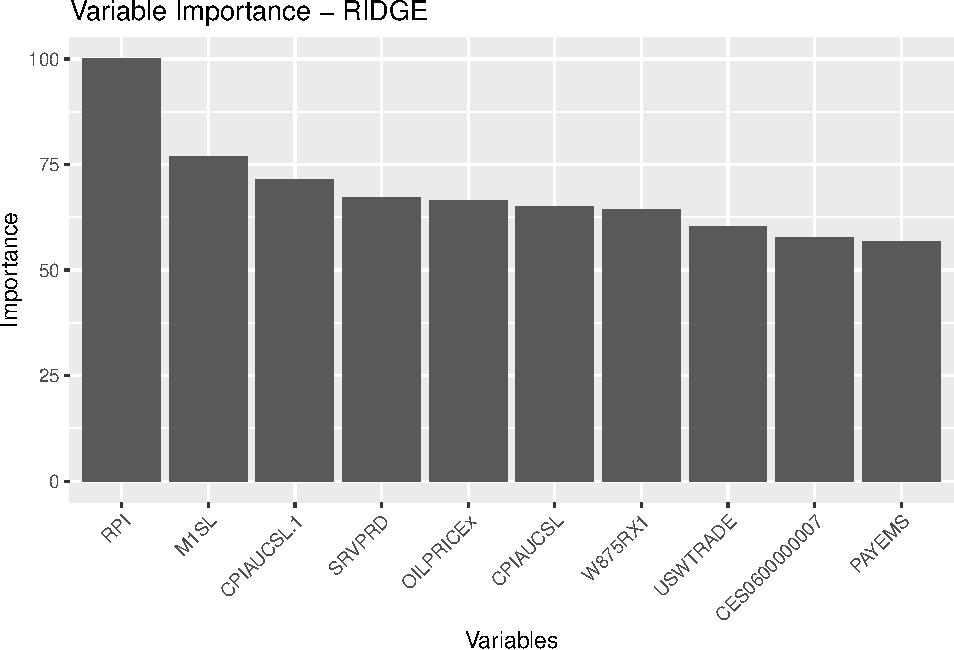
\includegraphics{Trabalho_Econo4_Q2_files/figure-latex/unnamed-chunk-29-1.pdf}

We now compute importance by group in Ridge.

\begin{Shaded}
\begin{Highlighting}[]
\CommentTok{\# Get sum over groups Sum over cells based on groups}

\NormalTok{ridge\_coeff\_std }\OtherTok{\textless{}{-}}\NormalTok{ ridge\_coeff\_std }\SpecialCharTok{\%\textgreater{}\%}
    \FunctionTok{rename}\NormalTok{(}\AttributeTok{fred =} \StringTok{"ridge\_names"}\NormalTok{)}

\NormalTok{ridge\_coeff\_std }\OtherTok{\textless{}{-}} \FunctionTok{merge}\NormalTok{(ridge\_coeff\_std, groups, }\AttributeTok{by =} \StringTok{"fred"}\NormalTok{,}
    \AttributeTok{all.x =} \ConstantTok{TRUE}\NormalTok{)}

\NormalTok{ridge\_group }\OtherTok{\textless{}{-}}\NormalTok{ ridge\_coeff\_std}

\ControlFlowTok{for}\NormalTok{ (i }\ControlFlowTok{in} \DecValTok{2}\SpecialCharTok{:}\DecValTok{262}\NormalTok{) \{}
    \ControlFlowTok{for}\NormalTok{ (j }\ControlFlowTok{in} \DecValTok{1}\SpecialCharTok{:}\DecValTok{108}\NormalTok{) \{}
\NormalTok{        ridge\_group[j, i] }\OtherTok{\textless{}{-}} \FunctionTok{abs}\NormalTok{(ridge\_coeff\_std[j, i])}\SpecialCharTok{/}\FunctionTok{sum}\NormalTok{(}\FunctionTok{abs}\NormalTok{((ridge\_coeff\_std[,}
\NormalTok{            i])))}
\NormalTok{    \}}
\NormalTok{\}}

\NormalTok{group\_sums }\OtherTok{\textless{}{-}}\NormalTok{ ridge\_group }\SpecialCharTok{\%\textgreater{}\%}
    \FunctionTok{group\_by}\NormalTok{(group) }\SpecialCharTok{\%\textgreater{}\%}
    \FunctionTok{summarize}\NormalTok{(}\FunctionTok{across}\NormalTok{(}\DecValTok{2}\SpecialCharTok{:}\DecValTok{262}\NormalTok{, }\SpecialCharTok{\textasciitilde{}}\FunctionTok{sum}\NormalTok{(.)))}

\FunctionTok{colnames}\NormalTok{(group\_sums)[}\DecValTok{2}\SpecialCharTok{:}\DecValTok{262}\NormalTok{] }\OtherTok{\textless{}{-}} \FunctionTok{as.Date}\NormalTok{(}\FunctionTok{time}\NormalTok{(forecast1))}

\NormalTok{group\_sums\_long }\OtherTok{\textless{}{-}} \FunctionTok{pivot\_longer}\NormalTok{(group\_sums, }\AttributeTok{cols =} \SpecialCharTok{{-}}\NormalTok{group, }\AttributeTok{names\_to =} \StringTok{"Time"}\NormalTok{,}
    \AttributeTok{values\_to =} \StringTok{"Value"}\NormalTok{)}
\NormalTok{group\_sums\_long}\SpecialCharTok{$}\NormalTok{Time }\OtherTok{\textless{}{-}} \FunctionTok{as.integer}\NormalTok{(group\_sums\_long}\SpecialCharTok{$}\NormalTok{Time)}
\NormalTok{group\_sums\_long}\SpecialCharTok{$}\NormalTok{date }\OtherTok{\textless{}{-}} \FunctionTok{as.Date}\NormalTok{(group\_sums\_long}\SpecialCharTok{$}\NormalTok{Time)}

\FunctionTok{ggplot}\NormalTok{(group\_sums\_long, }\FunctionTok{aes}\NormalTok{(}\AttributeTok{x =}\NormalTok{ date, }\AttributeTok{y =}\NormalTok{ Value, }\AttributeTok{fill =} \FunctionTok{factor}\NormalTok{(group))) }\SpecialCharTok{+}
    \FunctionTok{geom\_area}\NormalTok{() }\SpecialCharTok{+} \FunctionTok{labs}\NormalTok{(}\AttributeTok{title =} \StringTok{"RIDGE {-} Group Importance over Time"}\NormalTok{,}
    \AttributeTok{x =} \StringTok{"Time"}\NormalTok{, }\AttributeTok{y =} \StringTok{"Relative Values"}\NormalTok{) }\SpecialCharTok{+} \FunctionTok{scale\_fill\_discrete}\NormalTok{(}\AttributeTok{name =} \StringTok{"Groups"}\NormalTok{) }\SpecialCharTok{+}
    \FunctionTok{theme\_bw}\NormalTok{() }\SpecialCharTok{+} \FunctionTok{scale\_fill\_jco}\NormalTok{()}
\end{Highlighting}
\end{Shaded}

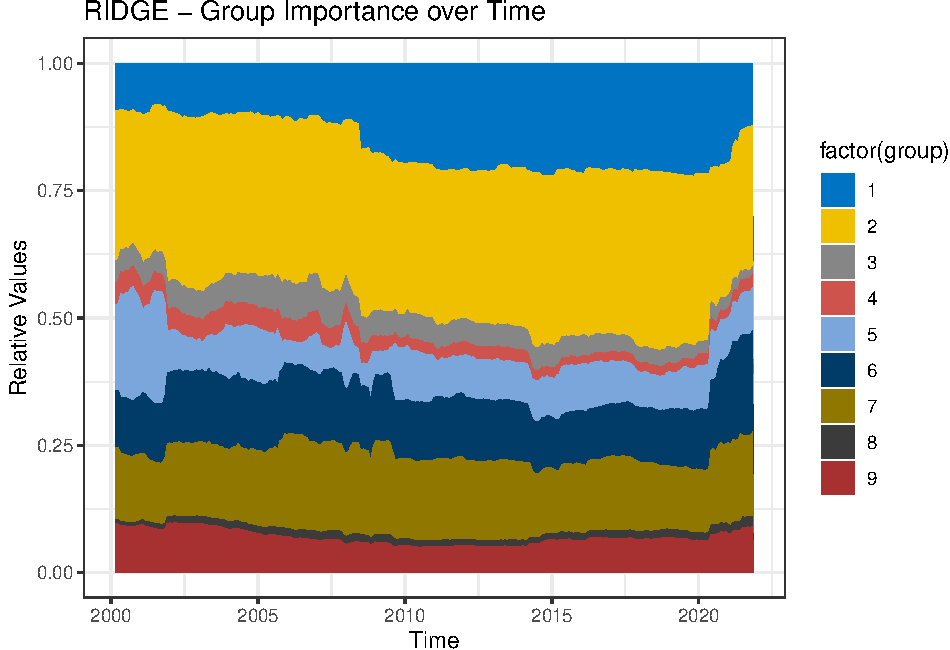
\includegraphics{Trabalho_Econo4_Q2_files/figure-latex/unnamed-chunk-30-1.pdf}
We repeat the exercise for LASSO. First selecting the top 10 most
important variables.

\begin{Shaded}
\begin{Highlighting}[]
\CommentTok{\# Computing variable importance for LASSO}

\CommentTok{\# Create a matrix to store coefficients}

\NormalTok{coeff\_lasso }\OtherTok{\textless{}{-}} \FunctionTok{data.frame}\NormalTok{(}\FunctionTok{matrix}\NormalTok{(}\AttributeTok{ncol =} \FunctionTok{ncol}\NormalTok{(reg\_data2), }\AttributeTok{nrow =} \FunctionTok{length}\NormalTok{(forecast1)))}
\FunctionTok{colnames}\NormalTok{(coeff\_lasso) }\OtherTok{\textless{}{-}} \FunctionTok{colnames}\NormalTok{(reg\_data2)}

\CommentTok{\# Retrieve coefficients and variable identifiers from lists}
\NormalTok{var\_lasso }\OtherTok{=} \FunctionTok{modify\_depth}\NormalTok{(coefficients\_lasso, }\DecValTok{1}\NormalTok{, }\StringTok{"i"}\NormalTok{)}
\NormalTok{co\_lasso }\OtherTok{=} \FunctionTok{modify\_depth}\NormalTok{(coefficients\_lasso, }\DecValTok{1}\NormalTok{, }\StringTok{"x"}\NormalTok{)}

\ControlFlowTok{for}\NormalTok{ (i }\ControlFlowTok{in} \DecValTok{1}\SpecialCharTok{:}\FunctionTok{length}\NormalTok{(forecast1)) \{}
\NormalTok{    a }\OtherTok{=}\NormalTok{ var\_lasso[[i]] }\SpecialCharTok{\%\textgreater{}\%}
        \FunctionTok{unlist}\NormalTok{()}
\NormalTok{    b }\OtherTok{=}\NormalTok{ co\_lasso[[i]] }\SpecialCharTok{\%\textgreater{}\%}
        \FunctionTok{unlist}\NormalTok{()}
    \ControlFlowTok{for}\NormalTok{ (c }\ControlFlowTok{in} \DecValTok{2}\SpecialCharTok{:}\FunctionTok{length}\NormalTok{(a)) \{}
\NormalTok{        coeff\_lasso[i, a[c]] }\OtherTok{\textless{}{-}}\NormalTok{ b[c]}
\NormalTok{    \}}
\NormalTok{\}}

\FunctionTok{rm}\NormalTok{(var\_lasso, co\_lasso)}

\CommentTok{\# Multiply for sd}
\ControlFlowTok{for}\NormalTok{ (i }\ControlFlowTok{in} \DecValTok{1}\SpecialCharTok{:}\FunctionTok{length}\NormalTok{(forecast1)) \{}
\NormalTok{    coeff\_lasso[, i] }\OtherTok{=}\NormalTok{ coeff\_lasso[, i] }\SpecialCharTok{*} \FunctionTok{sd}\NormalTok{(reg\_data2[, i])}
\NormalTok{\}}
\end{Highlighting}
\end{Shaded}

We compute the 10 most relevant predictors considering the mean absolute
value of the coefficients over all estimation windows.

\begin{Shaded}
\begin{Highlighting}[]
\NormalTok{coeff\_lasso }\OtherTok{\textless{}{-}}\NormalTok{ coeff\_lasso }\SpecialCharTok{\%\textgreater{}\%}
    \FunctionTok{mutate\_all}\NormalTok{(}\SpecialCharTok{\textasciitilde{}}\FunctionTok{replace\_na}\NormalTok{(., }\DecValTok{0}\NormalTok{))}

\NormalTok{top10\_lasso }\OtherTok{\textless{}{-}} \FunctionTok{colMeans}\NormalTok{(}\FunctionTok{abs}\NormalTok{(coeff\_lasso))}

\NormalTok{top\_10\_lasso }\OtherTok{\textless{}{-}}\NormalTok{ coeff\_lasso }\SpecialCharTok{\%\textgreater{}\%}
    \FunctionTok{summarise\_all}\NormalTok{(}\SpecialCharTok{\textasciitilde{}}\FunctionTok{mean}\NormalTok{(}\FunctionTok{abs}\NormalTok{(.))) }\SpecialCharTok{\%\textgreater{}\%}
    \FunctionTok{pivot\_longer}\NormalTok{(}\FunctionTok{everything}\NormalTok{()) }\SpecialCharTok{\%\textgreater{}\%}
    \FunctionTok{arrange}\NormalTok{(}\FunctionTok{desc}\NormalTok{(value)) }\SpecialCharTok{\%\textgreater{}\%}
    \FunctionTok{head}\NormalTok{(}\DecValTok{10}\NormalTok{)}

\NormalTok{top\_10\_lasso }\OtherTok{\textless{}{-}}\NormalTok{ top\_10\_lasso }\SpecialCharTok{\%\textgreater{}\%}
    \FunctionTok{mutate}\NormalTok{(}\AttributeTok{importance =} \DecValTok{100} \SpecialCharTok{*}\NormalTok{ value}\SpecialCharTok{/}\NormalTok{value[}\DecValTok{1}\NormalTok{]) }\SpecialCharTok{\%\textgreater{}\%}
    \FunctionTok{arrange}\NormalTok{(}\FunctionTok{desc}\NormalTok{(importance))}

\FunctionTok{ggplot}\NormalTok{(top\_10\_lasso, }\FunctionTok{aes}\NormalTok{(}\AttributeTok{x =} \FunctionTok{reorder}\NormalTok{(name, }\SpecialCharTok{{-}}\NormalTok{importance), }\AttributeTok{y =}\NormalTok{ importance)) }\SpecialCharTok{+}
    \FunctionTok{geom\_bar}\NormalTok{(}\AttributeTok{stat =} \StringTok{"identity"}\NormalTok{) }\SpecialCharTok{+} \FunctionTok{labs}\NormalTok{(}\AttributeTok{title =} \StringTok{"Variable Importance {-} LASSO"}\NormalTok{,}
    \AttributeTok{x =} \StringTok{"Variables"}\NormalTok{, }\AttributeTok{y =} \StringTok{"Importance"}\NormalTok{) }\SpecialCharTok{+} \FunctionTok{theme}\NormalTok{(}\AttributeTok{axis.text.x =} \FunctionTok{element\_text}\NormalTok{(}\AttributeTok{angle =} \DecValTok{45}\NormalTok{,}
    \AttributeTok{hjust =} \DecValTok{1}\NormalTok{))}
\end{Highlighting}
\end{Shaded}

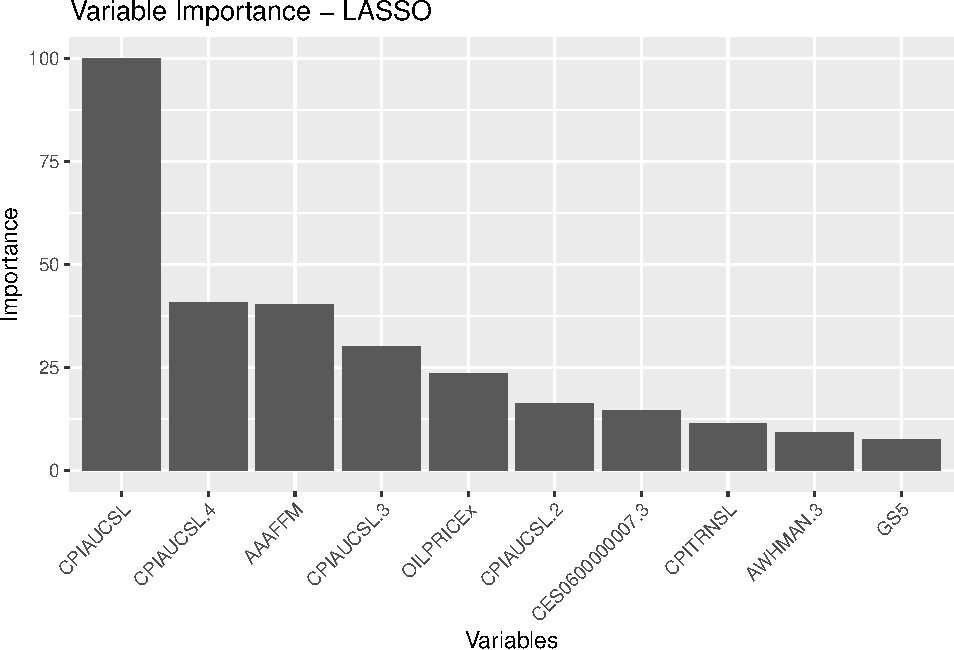
\includegraphics{Trabalho_Econo4_Q2_files/figure-latex/unnamed-chunk-32-1.pdf}
We now present results for groups. Group 9 (previous inflation) is
consistently the most important though less important throught the
sample. Groups 6 (bond and exchange rates) and 7 (prices) are important.
Group (2) labor market used to be relevant. For the most recent windows,
not so much.

\begin{Shaded}
\begin{Highlighting}[]
\CommentTok{\# Get sum over groups Sum over cells based on groups}
\NormalTok{coeff\_long }\OtherTok{\textless{}{-}} \FunctionTok{data.frame}\NormalTok{(}\AttributeTok{variable =} \FunctionTok{rep}\NormalTok{(}\FunctionTok{colnames}\NormalTok{(coeff\_lasso),}
    \AttributeTok{each =} \FunctionTok{nrow}\NormalTok{(coeff\_lasso)), }\AttributeTok{row\_index =} \FunctionTok{rep}\NormalTok{(}\DecValTok{1}\SpecialCharTok{:}\FunctionTok{nrow}\NormalTok{(coeff\_lasso),}
    \AttributeTok{times =} \FunctionTok{ncol}\NormalTok{(coeff\_lasso)), }\AttributeTok{value =} \FunctionTok{as.vector}\NormalTok{(}\FunctionTok{as.matrix}\NormalTok{(coeff\_lasso)))}

\NormalTok{coeff\_long }\OtherTok{\textless{}{-}}\NormalTok{ coeff\_long }\SpecialCharTok{\%\textgreater{}\%}
    \FunctionTok{arrange}\NormalTok{(row\_index)}
\NormalTok{groups }\OtherTok{\textless{}{-}}\NormalTok{ groups }\SpecialCharTok{\%\textgreater{}\%}
    \FunctionTok{rename}\NormalTok{(}\AttributeTok{variable =} \StringTok{"fred"}\NormalTok{)}
\NormalTok{merged\_data }\OtherTok{\textless{}{-}} \FunctionTok{merge}\NormalTok{(coeff\_long, groups, }\AttributeTok{by =} \StringTok{"variable"}\NormalTok{, }\AttributeTok{all.x =} \ConstantTok{TRUE}\NormalTok{)}
\NormalTok{merged\_data }\OtherTok{\textless{}{-}}\NormalTok{ merged\_data }\SpecialCharTok{\%\textgreater{}\%}
    \FunctionTok{arrange}\NormalTok{(row\_index)}

\NormalTok{groupfinal\_lasso }\OtherTok{\textless{}{-}}\NormalTok{ merged\_data }\SpecialCharTok{\%\textgreater{}\%}
    \FunctionTok{group\_by}\NormalTok{(row\_index, group) }\SpecialCharTok{\%\textgreater{}\%}
    \FunctionTok{summarise}\NormalTok{(}\AttributeTok{total =} \FunctionTok{sum}\NormalTok{(}\FunctionTok{abs}\NormalTok{(value)))}

\NormalTok{wide\_group\_lasso }\OtherTok{\textless{}{-}}\NormalTok{ groupfinal\_lasso }\SpecialCharTok{\%\textgreater{}\%}
    \FunctionTok{pivot\_wider}\NormalTok{(}\AttributeTok{names\_from =}\NormalTok{ group, }\AttributeTok{values\_from =}\NormalTok{ total) }\SpecialCharTok{\%\textgreater{}\%}
    \FunctionTok{ungroup}\NormalTok{()}

\NormalTok{wide\_group\_lasso\_rel }\OtherTok{\textless{}{-}}\NormalTok{ wide\_group\_lasso }\SpecialCharTok{\%\textgreater{}\%}
    \FunctionTok{mutate}\NormalTok{(}\FunctionTok{across}\NormalTok{(}\SpecialCharTok{{-}}\DecValTok{1}\NormalTok{, }\SpecialCharTok{\textasciitilde{}}\NormalTok{.}\SpecialCharTok{/}\FunctionTok{rowSums}\NormalTok{(}\FunctionTok{across}\NormalTok{(}\SpecialCharTok{{-}}\DecValTok{1}\NormalTok{))))}

\NormalTok{wide\_group\_lasso\_rel}\SpecialCharTok{$}\NormalTok{dates }\OtherTok{\textless{}{-}} \FunctionTok{as.Date}\NormalTok{(}\FunctionTok{time}\NormalTok{(forecast1))}

\CommentTok{\# Melt the dataframe to long format for plotting}
\NormalTok{melted\_df }\OtherTok{\textless{}{-}} \FunctionTok{melt}\NormalTok{(wide\_group\_lasso\_rel, }\AttributeTok{id.vars =} \StringTok{"dates"}\NormalTok{, }\AttributeTok{variable.name =} \StringTok{"Column"}\NormalTok{)}
\NormalTok{melted\_df }\OtherTok{\textless{}{-}}\NormalTok{ melted\_df }\SpecialCharTok{\%\textgreater{}\%}
    \FunctionTok{filter}\NormalTok{(Column }\SpecialCharTok{!=} \StringTok{"row\_index"}\NormalTok{)}
\NormalTok{melted\_df}\SpecialCharTok{$}\NormalTok{Group }\OtherTok{\textless{}{-}} \FunctionTok{as.integer}\NormalTok{(melted\_df}\SpecialCharTok{$}\NormalTok{Column) }\SpecialCharTok{{-}} \DecValTok{1}
\NormalTok{melted\_df}\SpecialCharTok{$}\NormalTok{Group }\OtherTok{\textless{}{-}} \FunctionTok{as.character}\NormalTok{(melted\_df}\SpecialCharTok{$}\NormalTok{Group)}


\CommentTok{\# Create a stacked column plot}
\FunctionTok{ggplot}\NormalTok{(}\AttributeTok{data =}\NormalTok{ melted\_df, }\FunctionTok{aes}\NormalTok{(}\AttributeTok{x =}\NormalTok{ dates, }\AttributeTok{y =}\NormalTok{ value, }\AttributeTok{fill =}\NormalTok{ Group)) }\SpecialCharTok{+}
    \FunctionTok{geom\_area}\NormalTok{() }\SpecialCharTok{+} \FunctionTok{labs}\NormalTok{(}\AttributeTok{title =} \StringTok{"LASSO {-} Group Importance over Time"}\NormalTok{,}
    \AttributeTok{x =} \StringTok{"Time"}\NormalTok{, }\AttributeTok{y =} \StringTok{"Relative Values"}\NormalTok{) }\SpecialCharTok{+} \FunctionTok{scale\_fill\_discrete}\NormalTok{(}\AttributeTok{name =} \StringTok{"Groups"}\NormalTok{) }\SpecialCharTok{+}
    \FunctionTok{theme\_minimal}\NormalTok{() }\SpecialCharTok{+} \FunctionTok{scale\_fill\_jco}\NormalTok{()}
\end{Highlighting}
\end{Shaded}

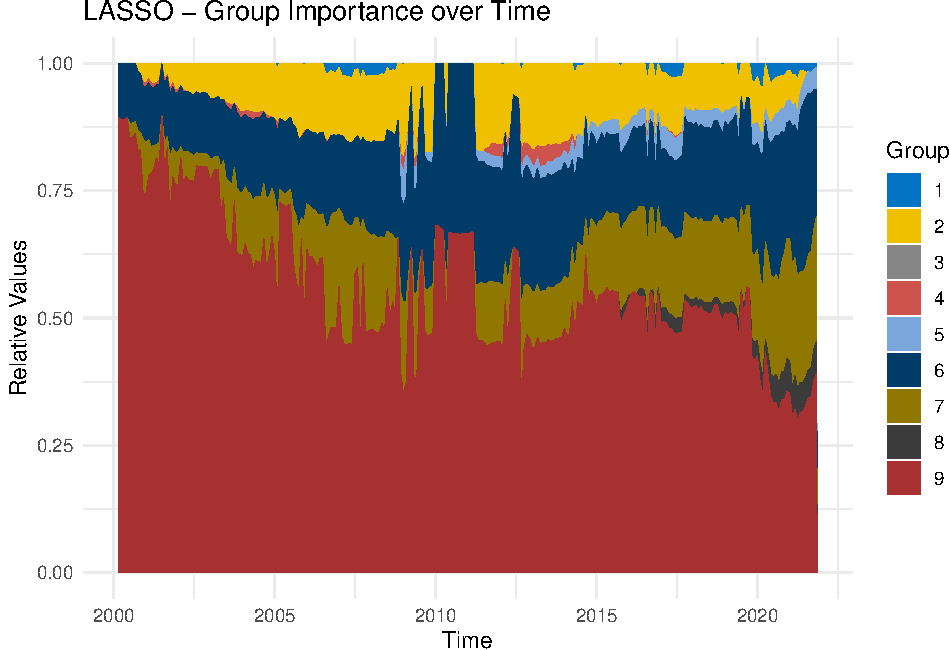
\includegraphics{Trabalho_Econo4_Q2_files/figure-latex/unnamed-chunk-33-1.pdf}
Finally, we do that for the AR+PC model, computing variable importance
of the PC block of the model. This is slightly more complicated than
LASSO and Ridge. We retrieve the alphas from the Factor on Variables and
then multiply them be the coefficients in the model regression.

\begin{Shaded}
\begin{Highlighting}[]
\CommentTok{\# Computing variable importance for PC}

\CommentTok{\# Get the alphas}
\NormalTok{alpha }\OtherTok{=} \FunctionTok{as.matrix}\NormalTok{(pca}\SpecialCharTok{$}\NormalTok{rotation[, }\DecValTok{1}\SpecialCharTok{:}\NormalTok{n\_pc])}

\CommentTok{\# Get the lambdas (coefficients of the Factors) and the}
\CommentTok{\# phis}
\NormalTok{lambdas }\OtherTok{=} \FunctionTok{matrix}\NormalTok{(}\ConstantTok{NA}\NormalTok{, }\DecValTok{261}\NormalTok{, }\DecValTok{6}\NormalTok{)}
\NormalTok{phis }\OtherTok{=} \FunctionTok{matrix}\NormalTok{(}\ConstantTok{NA}\NormalTok{, }\DecValTok{261}\NormalTok{, }\DecValTok{24}\NormalTok{)}

\ControlFlowTok{for}\NormalTok{ (i }\ControlFlowTok{in} \DecValTok{1}\SpecialCharTok{:}\DecValTok{261}\NormalTok{) \{}
\NormalTok{    size }\OtherTok{=} \FunctionTok{length}\NormalTok{(coefficients\_pc1[[i]])}
\NormalTok{    lags }\OtherTok{=}\NormalTok{ size }\SpecialCharTok{{-}} \DecValTok{1} \SpecialCharTok{{-}} \DecValTok{6}  \CommentTok{\# intercept and 6 factors}
    \ControlFlowTok{for}\NormalTok{ (j }\ControlFlowTok{in} \DecValTok{1}\SpecialCharTok{:}\DecValTok{6}\NormalTok{) \{}
\NormalTok{        lambdas[i, j] }\OtherTok{\textless{}{-}}\NormalTok{ coefficients\_pc1[[i]][size }\SpecialCharTok{{-}} \DecValTok{6} \SpecialCharTok{+}\NormalTok{ j]}
\NormalTok{    \}}
    \ControlFlowTok{for}\NormalTok{ (l }\ControlFlowTok{in} \DecValTok{1}\SpecialCharTok{:}\DecValTok{24}\NormalTok{) \{}
\NormalTok{        phis[i, l] }\OtherTok{\textless{}{-}}\NormalTok{ coefficients\_pc1[[i]][l }\SpecialCharTok{+} \DecValTok{1}\NormalTok{]}
\NormalTok{    \}}
\NormalTok{\}}

\CommentTok{\# Multiply alpha by lambdas to get \textquotesingle{}coefficient\textquotesingle{} of each}
\CommentTok{\# variable in each window}
\NormalTok{importpc }\OtherTok{=} \FunctionTok{as.data.frame}\NormalTok{(alpha }\SpecialCharTok{\%*\%} \FunctionTok{t}\NormalTok{(lambdas))}
\NormalTok{phist }\OtherTok{=} \FunctionTok{as.data.frame}\NormalTok{(}\FunctionTok{t}\NormalTok{(phis))}
\NormalTok{row\_names }\OtherTok{\textless{}{-}} \FunctionTok{paste}\NormalTok{(}\StringTok{"CPIAUCSL"}\NormalTok{, }\FunctionTok{seq}\NormalTok{(}\DecValTok{1}\NormalTok{, }\DecValTok{24}\NormalTok{), }\AttributeTok{sep =} \StringTok{"."}\NormalTok{)}
\NormalTok{importpc}\SpecialCharTok{$}\NormalTok{fred }\OtherTok{=} \FunctionTok{rownames}\NormalTok{(importpc)}
\NormalTok{phist}\SpecialCharTok{$}\NormalTok{fred }\OtherTok{=}\NormalTok{ row\_names}
\NormalTok{importpc }\OtherTok{\textless{}{-}} \FunctionTok{rbind}\NormalTok{(importpc, phist)}

\NormalTok{groups }\OtherTok{\textless{}{-}}\NormalTok{ groups }\SpecialCharTok{\%\textgreater{}\%}
    \FunctionTok{rename}\NormalTok{(}\AttributeTok{fred =} \StringTok{"variable"}\NormalTok{)}
\NormalTok{importpc }\OtherTok{=} \FunctionTok{merge}\NormalTok{(importpc, groups, }\AttributeTok{by =} \StringTok{"fred"}\NormalTok{, }\AttributeTok{all.x =} \ConstantTok{TRUE}\NormalTok{)}
\NormalTok{importpc}\SpecialCharTok{$}\NormalTok{group }\OtherTok{\textless{}{-}} \FunctionTok{ifelse}\NormalTok{(}\FunctionTok{is.na}\NormalTok{(importpc}\SpecialCharTok{$}\NormalTok{group), }\DecValTok{9}\NormalTok{, importpc}\SpecialCharTok{$}\NormalTok{group)  }\CommentTok{\# giving all lags of inflation group 9}


\CommentTok{\# Get the number of lags {-} we use this in item A}
\NormalTok{lags\_PC\_AR }\OtherTok{\textless{}{-}} \FunctionTok{table}\NormalTok{(}\FunctionTok{colSums}\NormalTok{(}\SpecialCharTok{!}\FunctionTok{is.na}\NormalTok{(phist)))}

\NormalTok{lags\_PC\_AR }\OtherTok{\textless{}{-}} \FunctionTok{data.frame}\NormalTok{(}\AttributeTok{lags =} \FunctionTok{as.numeric}\NormalTok{(}\FunctionTok{names}\NormalTok{(lags\_PC\_AR)),}
    \AttributeTok{count =} \FunctionTok{as.numeric}\NormalTok{(lags\_PC\_AR))}

\NormalTok{lags\_PC\_AR }\OtherTok{=}\NormalTok{ lags\_PC\_AR[}\DecValTok{1}\SpecialCharTok{:}\DecValTok{13}\NormalTok{, ]}
\NormalTok{lags\_PC\_AR }\OtherTok{\textless{}{-}}\NormalTok{ lags\_PC\_AR }\SpecialCharTok{\%\textgreater{}\%}
    \FunctionTok{arrange}\NormalTok{(}\FunctionTok{desc}\NormalTok{(count))}
\end{Highlighting}
\end{Shaded}

Top 10 most relevant variables

\begin{Shaded}
\begin{Highlighting}[]
\NormalTok{top\_10\_pc }\OtherTok{\textless{}{-}}\NormalTok{ importpc }\SpecialCharTok{\%\textgreater{}\%}
    \FunctionTok{rowwise}\NormalTok{() }\SpecialCharTok{\%\textgreater{}\%}
    \FunctionTok{mutate}\NormalTok{(}\AttributeTok{mean\_abs =} \FunctionTok{mean}\NormalTok{(}\FunctionTok{abs}\NormalTok{(}\FunctionTok{c\_across}\NormalTok{(}\SpecialCharTok{{-}}\FunctionTok{c}\NormalTok{(fred, group))))) }\SpecialCharTok{\%\textgreater{}\%}
    \FunctionTok{ungroup}\NormalTok{() }\SpecialCharTok{\%\textgreater{}\%}
    \FunctionTok{select}\NormalTok{(fred, mean\_abs) }\SpecialCharTok{\%\textgreater{}\%}
    \FunctionTok{arrange}\NormalTok{(}\FunctionTok{desc}\NormalTok{(mean\_abs)) }\SpecialCharTok{\%\textgreater{}\%}
    \FunctionTok{head}\NormalTok{(}\DecValTok{10}\NormalTok{)}

\NormalTok{top\_10\_pc }\OtherTok{\textless{}{-}}\NormalTok{ top\_10\_pc }\SpecialCharTok{\%\textgreater{}\%}
    \FunctionTok{mutate}\NormalTok{(}\AttributeTok{importance =} \DecValTok{100} \SpecialCharTok{*}\NormalTok{ mean\_abs}\SpecialCharTok{/}\NormalTok{mean\_abs[}\DecValTok{1}\NormalTok{]) }\SpecialCharTok{\%\textgreater{}\%}
    \FunctionTok{arrange}\NormalTok{(}\FunctionTok{desc}\NormalTok{(importance))}

\FunctionTok{ggplot}\NormalTok{(top\_10\_pc, }\FunctionTok{aes}\NormalTok{(}\AttributeTok{x =} \FunctionTok{reorder}\NormalTok{(fred, }\SpecialCharTok{{-}}\NormalTok{importance), }\AttributeTok{y =}\NormalTok{ importance)) }\SpecialCharTok{+}
    \FunctionTok{geom\_bar}\NormalTok{(}\AttributeTok{stat =} \StringTok{"identity"}\NormalTok{) }\SpecialCharTok{+} \FunctionTok{labs}\NormalTok{(}\AttributeTok{title =} \StringTok{"Variable Importance {-} PC"}\NormalTok{,}
    \AttributeTok{x =} \StringTok{"Variables"}\NormalTok{, }\AttributeTok{y =} \StringTok{"Importance"}\NormalTok{) }\SpecialCharTok{+} \FunctionTok{theme}\NormalTok{(}\AttributeTok{axis.text.x =} \FunctionTok{element\_text}\NormalTok{(}\AttributeTok{angle =} \DecValTok{45}\NormalTok{,}
    \AttributeTok{hjust =} \DecValTok{1}\NormalTok{))}
\end{Highlighting}
\end{Shaded}

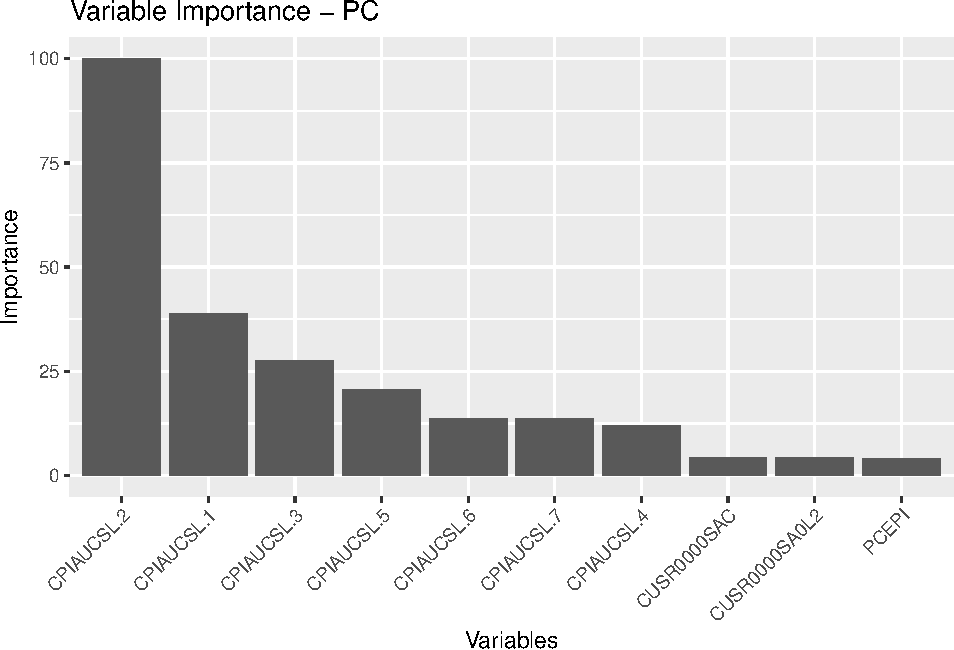
\includegraphics{Trabalho_Econo4_Q2_files/figure-latex/unnamed-chunk-35-1.pdf}
We again compute importance by group. Pattern is very close to that of
LASSO: Groups 9, 7, 6, 2

\begin{Shaded}
\begin{Highlighting}[]
\NormalTok{result }\OtherTok{\textless{}{-}}\NormalTok{ importpc }\SpecialCharTok{\%\textgreater{}\%}
    \FunctionTok{mutate}\NormalTok{(}\FunctionTok{across}\NormalTok{(}\FunctionTok{starts\_with}\NormalTok{(}\StringTok{"V"}\NormalTok{), }\SpecialCharTok{\textasciitilde{}}\FunctionTok{abs}\NormalTok{(.), }\AttributeTok{.names =} \StringTok{"abs\_\{.col\}"}\NormalTok{)) }\SpecialCharTok{\%\textgreater{}\%}
    \FunctionTok{group\_by}\NormalTok{(group) }\SpecialCharTok{\%\textgreater{}\%}
    \FunctionTok{summarise}\NormalTok{(}\FunctionTok{across}\NormalTok{(}\FunctionTok{starts\_with}\NormalTok{(}\StringTok{"abs\_V"}\NormalTok{), }\SpecialCharTok{\textasciitilde{}}\FunctionTok{sum}\NormalTok{(., }\AttributeTok{na.rm =} \ConstantTok{TRUE}\NormalTok{)))}

\NormalTok{pc\_rel }\OtherTok{\textless{}{-}}\NormalTok{ result }\SpecialCharTok{\%\textgreater{}\%}
    \FunctionTok{mutate}\NormalTok{(}\FunctionTok{across}\NormalTok{(}\FunctionTok{starts\_with}\NormalTok{(}\StringTok{"abs\_V"}\NormalTok{), }\SpecialCharTok{\textasciitilde{}}\NormalTok{.}\SpecialCharTok{/}\FunctionTok{sum}\NormalTok{(., }\AttributeTok{na.rm =} \ConstantTok{TRUE}\NormalTok{),}
        \AttributeTok{.names =} \StringTok{"rel\_\{.col\}"}\NormalTok{)) }\SpecialCharTok{\%\textgreater{}\%}
    \FunctionTok{select}\NormalTok{(}\FunctionTok{starts\_with}\NormalTok{(}\StringTok{"rel\_"}\NormalTok{))}

\NormalTok{pc\_rel\_transposed }\OtherTok{\textless{}{-}} \FunctionTok{as.data.frame}\NormalTok{((}\FunctionTok{t}\NormalTok{(pc\_rel)))}

\NormalTok{pc\_rel\_transposed }\OtherTok{\textless{}{-}}\NormalTok{ pc\_rel\_transposed }\SpecialCharTok{\%\textgreater{}\%}
    \FunctionTok{mutate}\NormalTok{(}\AttributeTok{date =} \FunctionTok{as.Date}\NormalTok{(}\FunctionTok{time}\NormalTok{(forecast1)))}

\NormalTok{importpc\_long }\OtherTok{\textless{}{-}}\NormalTok{ pc\_rel\_transposed }\SpecialCharTok{\%\textgreater{}\%}
    \FunctionTok{pivot\_longer}\NormalTok{(}\AttributeTok{cols =} \FunctionTok{starts\_with}\NormalTok{(}\StringTok{"V"}\NormalTok{), }\AttributeTok{names\_to =} \StringTok{"variable"}\NormalTok{,}
        \AttributeTok{values\_to =} \StringTok{"value"}\NormalTok{)}

\NormalTok{importpc\_long}\SpecialCharTok{$}\NormalTok{Group }\OtherTok{\textless{}{-}} \FunctionTok{as.character}\NormalTok{(}\FunctionTok{gsub}\NormalTok{(}\StringTok{"}\SpecialCharTok{\textbackslash{}\textbackslash{}}\StringTok{D"}\NormalTok{, }\StringTok{""}\NormalTok{, importpc\_long}\SpecialCharTok{$}\NormalTok{variable))}

\FunctionTok{ggplot}\NormalTok{(importpc\_long, }\FunctionTok{aes}\NormalTok{(}\AttributeTok{x =}\NormalTok{ date, }\AttributeTok{y =}\NormalTok{ value, }\AttributeTok{fill =}\NormalTok{ Group)) }\SpecialCharTok{+}
    \FunctionTok{geom\_area}\NormalTok{() }\SpecialCharTok{+} \FunctionTok{labs}\NormalTok{(}\AttributeTok{title =} \StringTok{"AR\_PC {-} Group Importance over Time"}\NormalTok{,}
    \AttributeTok{x =} \StringTok{"Time"}\NormalTok{, }\AttributeTok{y =} \StringTok{"Relative Values"}\NormalTok{) }\SpecialCharTok{+} \FunctionTok{scale\_fill\_discrete}\NormalTok{(}\AttributeTok{name =} \StringTok{"Groups"}\NormalTok{) }\SpecialCharTok{+}
    \FunctionTok{theme\_minimal}\NormalTok{() }\SpecialCharTok{+} \FunctionTok{scale\_fill\_jco}\NormalTok{()}
\end{Highlighting}
\end{Shaded}

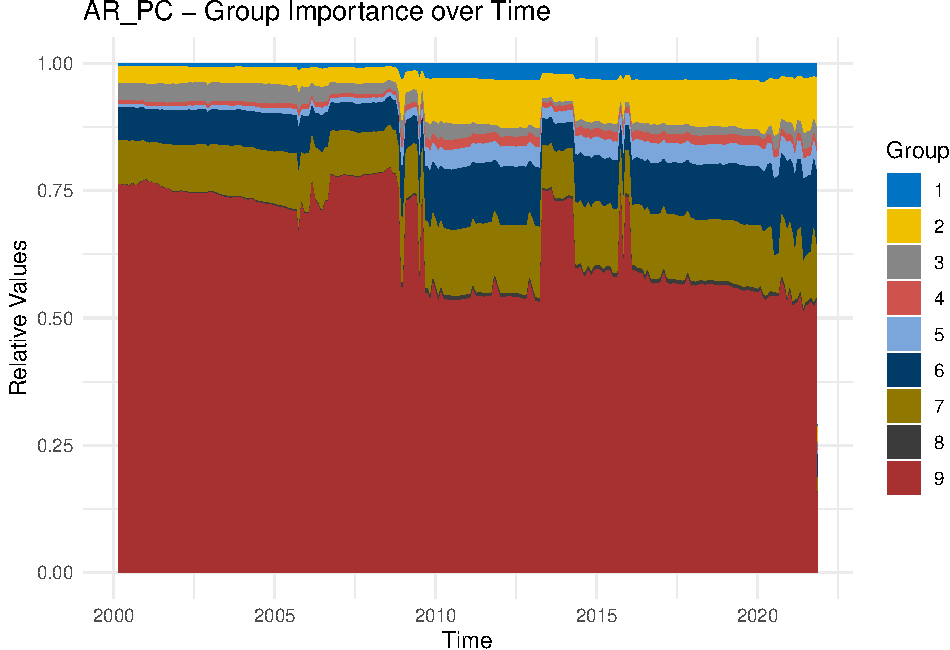
\includegraphics{Trabalho_Econo4_Q2_files/figure-latex/unnamed-chunk-36-1.pdf}

\end{document}
